%-----------------------------------------------------------------------------%
\chapter{IMPLEMENTASI DAN PENGUJIAN}
%-----------------------------------------------------------------------------%

%
\vspace{4.5pt}
\noindent Pada bab ini akan menjelaskan mengenai proses implementasi dan pengujian terhadap sistem yang telah dibangun berdasarkan penjelasan pada bab sebelumnya.\\

\section{Lingkungan Implementasi}
\noindent Pada lingkungan implementasi, akan dijelaskan mengenai perangkat yang digunakan dalam proses pembangunan sistem baik dari perangkat keras maupun perangkat lunak yang digunakan.\\

\subsection{Spesifikasi Perangkat Keras}
\noindent Spesifikasi dari perangkat keras yang digunakan dalam pembangunan aplikasi adalah sebagai berikut:
\begin{enumerate}
\item \textit{Laptop} ASUS A442UQ
\item \textit{Processor} Intel Core i7-7500U CPU @ 2.7GHz
\item \textit{Hard Disk} kapasitas 1TB
\item RAM 8GB\\
\end{enumerate}

\subsection{Lingkungan Perangkat Lunak}
\noindent Spesifikasi dari perangkat lunak yang digunakan dalam pembangunan aplikasi adalah sebagai berikut:
\begin{enumerate}
\item Sistem Operasi Windows 10 Home 64 bit.
\item Netbeans IDE 8.2
\item Java Development Kit (JDK) 1.8.0{\_}161
\item \textit{Library} OpenCV 3.4.6\\
\end{enumerate}

%\subsection{Penjelasan \textit{Dataset}}
%\noindent Pada implementasi digunakan dua buah \textit{dataset} yaitu \textit{Clothing Store} dan \textit{Outdoor}. Seperti yang telah dijelaskan pada bab 2, 80\% citra dari \textit{dataset Clothing Store} akan digunakan untuk pembelajaran dan 20\% citra lainya untuk pengujian. Sementara \textit{dataset Outdoor} yang terdiri atas 3 buah folder yaitu 31, 54, dan 56, di mana seluruh citra pada folder 56 untuk data belajar, lalu folder 31 dan folder 54 untuk data uji. Pada masing-masing \textit{dataset} didapatkan masing-masing citra positif yaitu berisi manusia sesuai dengan berkas \textit{ground truth} sedangkan citra negatif yaitu berisi selain manusia didapatkan secara acak yang tidak berpotongan dengan daerah citra manusia. Ukuran dari citra negatif adalah 65 $\times$ 80 piksel. Rincian dari jumlah citra, citra positif, dan citra negatif dapat dilihat pada tabel \ref{tbl:rincianDataset}.
%\begingroup
%\setlength{\LTleft}{-20cm plus -1fill}
%\setlength{\LTright}{\LTleft}
%\begin{small}
%\begin{longtable}{|c|c|c|c|c|c|c|}
%\caption{Rincian \textit{Dataset} untuk Implementasi}
%\label{tbl:rincianDataset}
%\endhead
%\hline
%\textit{\textbf{Dataset}}			& \textbf{Folder}			& \textbf{Keterangan}	& \textbf{Citra Belajar}	& \textbf{Citra Uji}	& \multicolumn{2}{c|}{\textbf{Total}} \\ \hline
%\multirow{3}{*}{\textit{Clothing Store}}	& \multirow{3}{*}{-}		& Citra				& 616					& 154				& \multicolumn{2}{c|}{770}            \\ \cline{3-7} 
%								&						& Manusia			& 1160					& 471				& 1631     & \multirow{2}{*}{5092}    \\ \cline{3-6}
%								&						& Lain-lain			& 2766					& 695				& 3461     &                          \\ \hline
%\multirow{9}{*}{\textit{Outdoor}}		& \multirow{3}{*}{31}	& Citra				& - 						& 46				& \multicolumn{2}{c|}{46}             \\ \cline{3-7} 
%								&						& Manusia			& - 						& 218				& 218      & \multirow{2}{*}{427}     \\ \cline{3-6}
%								&						& Lain-lain			& - 						& 209				& 209      &                          \\ \cline{2-7} 
%								& \multirow{3}{*}{54}	& Citra				& - 						& 84				& \multicolumn{2}{c|}{84}             \\ \cline{3-7} 
%								&						& Manusia			& - 						& 371				& 371      & \multirow{2}{*}{744}     \\ \cline{3-6}
%								&						& Lain-lain			& - 						& 373				& 373      &                          \\ \cline{2-7} 
%								& \multirow{3}{*}{56}	& Citra				& 113					& - 					& \multicolumn{2}{c|}{113}            \\ \cline{3-7} 
%								&						& Manusia			& 496					& - 					& 496      & \multirow{2}{*}{999}     \\ \cline{3-6}
%								&						& Lain-lain			& 503					& - 					& 503      &                          \\ \hline
%\end{longtable}
%\end{small}
%\endgroup

\section{Implementasi Perangkat Lunak}
\noindent Pada bab ini akan dijelaskan mengenai implementasi aplikasi untuk pengenalan karakter pada citra plat kendaraan. Di bawah ini merupakan daftar \textit{class} dan \textit{method} beserta penjelasan mengenai cara kerja program.\\
\subsection{Daftar \textit{Class} dan \textit{Method} Gradient}
\noindent Berikut adalah tabel berisi \textit{method} pada \textit{class} Gradient. \textit{Class} Gradient digunakan untuk menyimpan nilai \textit{orientation} dan nilai \textit{magnitude} dari suatu piksel citra.
\begin{small}
	\begin{longtable}{| p {0.5cm} | p {4.5cm} | p {4cm} | p {1.5cm} | p {3cm} |}
		\caption{Daftar \textit{Method Class Gradient} } \\
		\hline
		\textbf{No}  & \textbf{Nama \textit{method}}  & \textbf{Masukan}  & \textbf{Keluaran} & \textbf{Keterangan} \\
		\hline
		\endfirsthead
		\endhead	
		1	& Gradient & double orientation, double magnitude & void & Metode \textit{constructor} yang digunakan untuk inisialisasi objek dari kelas Gradient dengan nilai \textit{orientation} dan \textit{magnitude} yang didapatkan dari perhitungan. \\
		\hline
		2	& getOrientation() & & double & Metode untuk mengembalikan nilai \textit{orientation} dari suatu piksel.\\
		\hline
		3	& getMagnitude() & & double & Metode yang digunakan untuk mengembalikan nilai \textit{magnitude} dari suatu piksel.\\
		\hline
		4	& setOrientation() & double orientation & void & Metode untuk mengatur nilai \textit{orientation} dari objek Gradient berdasarkan nilai \textit{orientation} yang dijadikan masukkan.\\
		\hline
		5	& setMagnitude() & double magnitude & void & Metode yang digunakan untuk mengatur nilai \textit{magnitude} dari objek Gradient berdasarkan nilai \textit{magnitude}  yang dijadikan masukkan.\\
		\hline
	\end{longtable}
\end{small}

\subsection{Daftar \textit{Class} dan \textit{Method} GradientCell}
\noindent Berikut adalah tabel berisi \textit{method} pada \textit{class} GradientCell. \textit{Class} GradientCell digunakan untuk menyimpan nilai gradien dari setiap sel.
\begin{small}
	\begin{longtable}{| p {0.5cm} | p {4.5cm} | p {3cm} | p {2.5cm} | p {3cm} |}
		\caption{Daftar \textit{Method Class GradientCell} } \\
		\hline
		\textbf{No}  & \textbf{Nama \textit{method}}  & \textbf{Masukan}  & \textbf{Keluaran} & \textbf{Keterangan} \\
		\hline
		\endfirsthead
		\endhead	
		1	& GradientCell() & int length & void & Metode \textit{constructor} yang digunakan untuk inisialisasi objek dari kelas GradientCell. \\
		\hline
		2	& getGradients() & & List \textless Gradient \textgreater & Metode untuk mengembalikan \textit{List} dari gradien-gradien yang terdapat .\\
		\hline
	\end{longtable}
\end{small}

\subsection{Daftar \textit{Class} dan \textit{Method} HOG}
\noindent Berikut adalah tabel berisi \textit{method} pada \textit{class} HOG. \textit{Class} HOG digunakan untuk proses ekstraksi fitur dari citra karakter.
\begin{small}
	\begin{longtable}{| p {0.5cm} | p {4.5cm} | p {4cm} | p {1.5cm} | p {3cm} |}
		\caption{Daftar \textit{Method Class HOG} } \\
		\hline
		\textbf{No}  & \textbf{Nama \textit{method}}  & \textbf{Masukan}  & \textbf{Keluaran} & \textbf{Keterangan} \\
		\hline
		\endfirsthead
		\endhead	
		1	& HOG() & Integer[][] image, int cellHeight, int cellWidth, int blockSize, int numBins & void & Metode \textit{constructor} yang digunakan untuk inisialisasi objek dari kelas HOG. \\
		\hline
		2	& extractHOGFeatures() & & double[] & Metode untuk mengekstraksi fitur \textit{HOG descriptor} dari citra.\\
		\hline
		3	& calculateGradientAndCells() & & void & Metode yang digunakan untuk menghitung nilai gradien, \textit{magnitude}, dan orientasi untuk setiap sel.\\
		\hline
		4	& createHistograms() & 	& void & Metode untuk membentuk histogram untuk mencatat persebaran arah dari setiap sel.\\
		\hline
		5	& histogramNormalization() & & void & Melakukan normalisasi \textit{L2-Norm} untuk setiap elemen pada histogram.\\
		\hline
		6	& createDescriptor() & & void & Membentuk \textit{HOG descriptor} dari hasil normalisasi histogram.\\
		\hline
	\end{longtable}
\end{small}

\subsection{Daftar \textit{Class} dan \textit{Method} SVM}
\noindent Berikut adalah tabel berisi \textit{method} pada \textit{class} SVM. \textit{Class} SVM digunakan untuk perhitungan klasifikasi.
\begin{small}
	\begin{longtable}{| p {0.5cm} | p {4cm} | p {3cm} | p {3cm} | p {3cm} |}
		\caption{Daftar \textit{Method Class SVM} } \\
		\hline
		\textbf{No}  & \textbf{Nama \textit{method}}  & \textbf{Masukan}  & \textbf{Keluaran} & \textbf{Keterangan} \\
		\hline
		\endfirsthead
		\endhead	
		1	& calculateRBFKernel() & double[][] data, double sigma,
		int classSource, int classTarget	& double &	Menghitung nilai RBF Kernel.\\
		\hline
		2	& createRBFMatrix() & double[][] data, double[] sigma & double[][] & Membentuk matriks RBF dari data fitur.\\
		\hline
		3	& createLinearEquation() & double[][] rbfMatrix, double[] classList	& double[][]	& Membuat persamaan linear dari matriks RBF.\\
		\hline
		4	& getSolutions() & double[][] linearEquationMatix, double[] classList	& Matrix & Mendapatkan solusi dari persamaan linear yaitu nilai alpha dan bias.\\
		\hline
		5	& createRBFTestMatrix() & double[][] data, double sigma, double[] classList	& double & Membentuk matriks RBF untuk data pengujian.\\
		\hline
		6	& classify() & double[][] solutions, double[] rbfTest, double[] classList	& double & Mendapatkan nilai hasil klasifikasi berdasarkan data uji dan nilai alpha dan bias.\\
		\hline
		7	& getDataFromText() & String path	& double[][] & Membaca matriks fitur dari file teks.\\
		\hline
		
	\end{longtable}
\end{small}
%Package cnn
%\subsubsection{Daftar \textit{Class} dan \textit{Method}}
%\noindent \textit{Class} CNN merupakan kelas yang berfungsi untuk melaksanakan proses \textit{Convolutional Neural Network} dengan arsitektur lapisan dan \textit{hyperparameter} yang telah ditentukan, lihat tabel \ref{tbl:classCNN}.
%\begingroup
%\setlength{\LTleft}{-20cm plus -1fill}
%\setlength{\LTright}{\LTleft}
%\begin{small}
%\begin{longtable}{|p{0.4cm}|p{2cm}|p{1.8cm}|p{1.8cm}|p{1.7cm}|p{3.55cm}|}
%	\caption{Daftar \textit{Method} pada \textit{Class} CNN \label{tbl:classCNN}}\\
%	\hline
%	\multirow{2}{*}{\textbf{No}} & \multirow{2}{*}{\textit{\textbf{Method}}} & \multicolumn{2}{c|}{\textit{\textbf{Input}}} & \multirow{2}{*}{\textit{\textbf{Output}}} & 
%	\multirow{2}{*}{\textbf{Keterangan}}\\
%	\cline{3-4}
%	& & \textbf{Tipe} & \textbf{Variabel} & & \\
%	\endfirsthead
%	\multicolumn{6}{c}{\textbf{\tablename~\thetable} Daftar \textit{Method} pada \textit{Class} CNN (Lanjutan)} \\ \hline
%	\multirow{2}{*}{\textbf{No}} & \multirow{2}{*}{\textit{\textbf{Method}}} & \multicolumn{2}{c|}{\textit{\textbf{Input}}} & \multirow{2}{*}{\textit{\textbf{Output}}} & 
%	\multirow{2}{*}{\textbf{Keterangan}}\\
%	\cline{3-4}
%	& & \textbf{Tipe} & \textbf{Variabel} & & \\
%	\endhead
%	\hline
%	1 & CNN & List$<$\newline Layer$>$,\newline double,\newline double,\newline int,\newline String & layers,\newline alpha,\newline alphaDivider,\newline saveModel,\newline pathModel & - & Konstruktor yang menerima dan menyimpan nilai \textit{hyperparameter} serta melakukan inisialisasi nilai pada kelas CNN.\\
%	\hline
%	2 & train & List$<$\newline TrainImage\newline$>$,\newline int & trainImg,\newline epoch & - & Melakukan tahap pembelajaran dari citra dengan pengulangan sebanyak \textit{epoch} serta menyimpan hasil pembelajaran.\\
%	\hline
%	3 & train & TrainImage & trainImg & - & Melakukan tahap pembelajaran untuk 1 citra, tahap \textit{forward} dan \textit{backward} yang mencakup menghitung turunan atau gradien lalu memperbarui nilai parameter berdasarkan gradien masing-masing.\\
%	\hline
%	4 & forward & TrainImage,\newline Process & img,\newline process & - & Melakukan tahap \textit{forward} pada setiap lapisan dan menghitung hasil berdasarkan proses pelatihan atau pengujian.\\
%	\hline
%	5 &  setGradient & TrainImage & img & - & Melakukan perhitungan gradien pada setiap lapisan.\\
%	\hline
%	6 & getData & - & - & List$<Data>$ & Menambahkan seluruh data yang telah dihitung pada setiap lapisan pada sebuah kelas \textit{List}.\\
%	\hline
%	7 & updateParams & - & - & - & Memperbarui parameter bobot berdasarkan data yang telah didapatkan dalam bentuk \textit{List}.\\
%	\hline
%	8 & update & int,\newline double,\newline double[] & j,\newline gradient,\newline weight & - & Menambahkan nilai bobot sesuai dengan gradiennya.\\
%	\hline
%	9 & test & List$<$\newline TrainImage\newline $>$ & trainImg & double & Melakukan tahap \textit{forward} untuk setiap gambar dan mengembalikan nilai akurasi.\\
%	\hline
%	10 & isHuman & double[][],\newline double & img,\newline threshold & boolean & Menguji adanya citra manusia yang dibatasi dengan probabilitas hasil pengujian.\\
%	\hline
%\end{longtable}
%\end{small}
%\endgroup

%\subsubsection{\textit{Class} CNNLoader}
%\noindent \textit{Class} CNNLoader merupakan kelas yang berfungsi untuk melakukan penyimpanan serta pemuatan model hasil pembelajaran \textit{Convolutional Neural Network}, lihat tabel \ref{tbl:classCNNLoader}.
%\begingroup
%\setlength{\LTleft}{-20cm plus -1fill}
%\setlength{\LTright}{\LTleft}
%\begin{small}
%\begin{longtable}{|p{0.4cm}|p{2cm}|p{1.8cm}|p{1.8cm}|p{1.7cm}|p{3.55cm}|}
%	\caption{Daftar \textit{Method} pada \textit{Class} CNNLoader \label{tbl:classCNNLoader}}\\
%	\hline
%	\multirow{2}{*}{\textbf{No}} & \multirow{2}{*}{\textit{\textbf{Method}}} & \multicolumn{2}{c|}{\textit{\textbf{Input}}} & \multirow{2}{*}{\textit{\textbf{Output}}} & 
%	\multirow{2}{*}{\textbf{Keterangan}}\\
%	\cline{3-4}
%	& & \textbf{Tipe} & \textbf{Variabel} & & \\
%	\endfirsthead
%	\multicolumn{6}{c}{\textbf{\tablename~\thetable} Daftar \textit{Method} pada \textit{Class} CNNLoader (Lanjutan)} \\
%	\hline
%	\multirow{2}{*}{\textbf{No}} & \multirow{2}{*}{\textit{\textbf{Method}}} & \multicolumn{2}{c|}{\textit{\textbf{Input}}} & \multirow{2}{*}{\textit{\textbf{Output}}} & 
%	\multirow{2}{*}{\textbf{Keterangan}}\\
%	\cline{3-4}
%	& & \textbf{Tipe} & \textbf{Variabel} & & \\
%	\endhead
%	\hline
%	1 & saveModel & String,\newline CNN & fileName,\newline cnn & - & Menyimpan model \textit{Convolutional Neural Network} dengan nama yang telah ditentukan.\\
%	\hline
%	2 & loadModel & String & fileName & CNN & Memuat model \textit{Convolutional Neural Network} yang telah disimpan sebelumnya.\\
%	\hline
%\end{longtable}
%\end{small}
%\endgroup

%Package cnn.layer
%\subsubsection{\textit{Class} Data}
%\noindent \textit{Class} Data merupakan kelas yang berfungsi untuk menyimpan data yang digunakan pada tahap \textit{Convolutional Neural Network}, lihat tabel \ref{tbl:classData}.
%\begingroup
%\setlength{\LTleft}{-20cm plus -1fill}
%\setlength{\LTright}{\LTleft}
%\begin{small}
%\begin{longtable}{|p{0.4cm}|p{2cm}|p{1.8cm}|p{1.8cm}|p{1.7cm}|p{3.55cm}|}
%	\caption{Daftar \textit{Method} pada \textit{Class} Data \label{tbl:classData}}\\
%	\hline
%	\multirow{2}{*}{\textbf{No}} & \multirow{2}{*}{\textit{\textbf{Method}}} & \multicolumn{2}{c|}{\textit{\textbf{Input}}} & \multirow{2}{*}{\textit{\textbf{Output}}} & 
%	\multirow{2}{*}{\textbf{Keterangan}}\\
%	\cline{3-4}
%	& & \textbf{Tipe} & \textbf{Variabel} & & \\
%	\endfirsthead
%	\multicolumn{6}{c}{\textbf{\tablename~\thetable} Daftar \textit{Method} pada \textit{Class} Data (Lanjutan)} \\
%	\hline
%	\multirow{2}{*}{\textbf{No}} & \multirow{2}{*}{\textit{\textbf{Method}}} & \multicolumn{2}{c|}{\textit{\textbf{Input}}} & \multirow{2}{*}{\textit{\textbf{Output}}} & 
%	\multirow{2}{*}{\textbf{Keterangan}}\\
%	\cline{3-4}
%	& & \textbf{Tipe} & \textbf{Variabel} & & \\
%	\endhead
%	\hline
%	1 & Data & Size & size & - & Konstruktor yang menerima dan menyimpan besar ukuran.\\
%	\hline
%	2 & addImage-\newline Data & double[][] & trainImg & - & Menyimpan nilai dari citra.\\
%	\hline
%	3 & getSize & - & - & Size & Digunakan untuk mendapatkan ukuran dari data.\\
%	\hline
%	4 & getWeight & int & index & double & Digunakan untuk mendapatkan bobot pada indeks 1 dimensi.\\
%	\hline
%	5 & getWeight & int,\newline int,\newline int & x,\newline y,\newline depth & double & Digunakan untuk mendapatkan bobot pada indeks 3 dimensi.\\
%	\hline
%	6 & setWeight & double & value & - & Digunakan untuk mendapatkan bobot pada indeks 1 dimensi.\\
%	\hline
%	7 & setWeight & int,\newline int,\newline int,\newline double & x,\newline y,\newline depth,\newline value & - & Digunakan untuk menetapkan nilai bobot pada indeks 3 dimensi.\\
%	\hline
%	8 & addWeight & int,\newline int,\newline int,\newline double & x,\newline y,\newline depth,\newline value & - & Digunakan untuk menambahkan nilai bobot.\\
%	\hline
%	9 & getGradient & int,\newline int,\newline int & x,\newline y,\newline depth & double & Digunakan untuk mendapatkan ukuran dari data pada indeks 3 dimensi.\\
%	\hline
%	10 & getGradient & int & index & double & Digunakan untuk mendapatkan ukuran dari data pada indeks 1 dimensi\\
%	\hline
%	11 & setGradient & int,\newline int,\newline int,\newline double & x,\newline y,\newline depth,\newline value & - & Digunakan untuk menentukan nilai gradien pada indeks 3 dimensi.\\
%	\hline
%	12 & setGradient & int & value & - & Digunakan untuk menentukan nilai gradien pada indeks 1 dimensi.\\
%	\hline
%	13 & addGradient & int,\newline int,\newline int,\newline double & x,\newline y,\newline depth,\newline value & - & Digunakan untuk nambahkan nilai gradien dengan indeks 3 dimensi.\\
%	\hline
%	14 & addGradient & int,\newline double & index,\newline value & - & Digunakan untuk nambahkan nilai gradien pada indeks 1 dimensi.\\
%	\hline
%	15 & calculate-\newline Index & int,\newline int,\newline int & x,\newline y,\newline depth & int & Digunakan untuk mendapatkan indeks pada 1 dimensi.\\
%	\hline
%	16 & clearGradient & - & - & - & Digunakan untuk hapus seluruh gradien.\\
%	\hline
%	17 & getWeights & - & - & double[] & Digunakan untuk mendapatkan seluruh bobot.\\
%	\hline
%	18 & getGradients & - & - & double[] & Digunakan untuk mendapatkan seluruh gradien.\\
%	\hline
%\end{longtable}
%\end{small}
%\endgroup

%\subsubsection{\textit{Class} Size}
%\noindent \textit{Class} Size merupakan kelas yang berfungsi untuk menyimpan informasi ukuran lebar, tinggi, dan kedalaman. Penjelasan mengenai kelas ini dapat dilihat pada tabel \ref{tbl:classSize}.
%\begingroup
%\setlength{\LTleft}{-20cm plus -1fill}
%\setlength{\LTright}{\LTleft}
%\begin{small}
%\begin{longtable}{|p{0.4cm}|p{2cm}|p{1.8cm}|p{1.8cm}|p{1.7cm}|p{3.55cm}|}
%	\caption{Daftar \textit{Method} pada \textit{Class} Size \label{tbl:classSize}}\\
%	\hline
%	\multirow{2}{*}{\textbf{No}} & \multirow{2}{*}{\textit{\textbf{Method}}} & \multicolumn{2}{c|}{\textit{\textbf{Input}}} & \multirow{2}{*}{\textit{\textbf{Output}}} & 
%	\multirow{2}{*}{\textbf{Keterangan}}\\
%	\cline{3-4}
%	& & \textbf{Tipe} & \textbf{Variabel} & & \\
%	\endfirsthead
%	\multicolumn{6}{c}{\textbf{\tablename~\thetable} Daftar \textit{Method} pada \textit{Class} Size (Lanjutan)} \\
%	\hline
%	\multirow{2}{*}{\textbf{No}} & \multirow{2}{*}{\textit{\textbf{Method}}} & \multicolumn{2}{c|}{\textit{\textbf{Input}}} & \multirow{2}{*}{\textit{\textbf{Output}}} & 
%	\multirow{2}{*}{\textbf{Keterangan}}\\
%	\cline{3-4}
%	& & \textbf{Tipe} & \textbf{Variabel} & & \\
%	\endhead
%	\hline
%	1 & Size & - & - & - & Konstruktor kosong ketika objek dibuat tanpa parameter.\\
%	\hline
%	2 & Size & int,\newline int,\newline int & width,\newline height,\newline depth & - & Konstruktor yang menerima dan menerima informasi ukuran.\\
%	\hline
%	3 & getWidth & - & - & int & Digunakan untuk mendapatkan lebar citra.\\
%	\hline
%	2 & setWidth & int & width & - & Digunakan untuk menentukan lebar citra.\\
%	\hline
%	2 & getHeight & - & - & int & Digunakan untuk mendapatkan tinggi citra.\\
%	\hline
%	2 & setHeight & int & height & - & Digunakan untuk menentukan tinggi citra.\\
%	\hline
%	2 & getDepth & - & - & int & Digunakan untuk mendapatkan kedalaman citra.\\
%	\hline
%	2 & setDepth & int & depth & - & Digunakan untuk menentukan kedalaman citra.\\
%	\hline
%	2 & toString & - & - & String & Mengembalikan informasi ukuran dalam bentuk text.\\
%	\hline
%\end{longtable}
%\end{small}
%\endgroup

%Package cnn.layer
%\subsubsection{\textit{Class} Layer}
%\noindent \textit{Class} Layer merupakan sebuah kelas abstrak untuk lapisan pada \textit{Convolutional Neural Network}. Penjelasan mengenai kelas ini dapat dilihat pada tabel \ref{tbl:classLayer}.
%\begingroup
%\setlength{\LTleft}{-20cm plus -1fill}
%\setlength{\LTright}{\LTleft}
%\begin{small}
%\begin{longtable}{|p{0.4cm}|p{2cm}|p{1.8cm}|p{1.8cm}|p{1.7cm}|p{3.55cm}|}
%	\caption{Daftar \textit{Method} pada \textit{Class} Layer \label{tbl:classLayer}}\\
%	\hline
%	\multirow{2}{*}{\textbf{No}} & \multirow{2}{*}{\textit{\textbf{Method}}} & \multicolumn{2}{c|}{\textit{\textbf{Input}}} & \multirow{2}{*}{\textit{\textbf{Output}}} & 
%	\multirow{2}{*}{\textbf{Keterangan}}\\
%	\cline{3-4}
%	& & \textbf{Tipe} & \textbf{Variabel} & & \\
%	\endfirsthead
%	\multicolumn{6}{c}{\textbf{\tablename~\thetable} Daftar \textit{Method} pada \textit{Class} Layer (Lanjutan)} \\
%	\hline
%	\multirow{2}{*}{\textbf{No}} & \multirow{2}{*}{\textit{\textbf{Method}}} & \multicolumn{2}{c|}{\textit{\textbf{Input}}} & \multirow{2}{*}{\textit{\textbf{Output}}} & 
%	\multirow{2}{*}{\textbf{Keterangan}}\\
%	\cline{3-4}
%	& & \textbf{Tipe} & \textbf{Variabel} & & \\
%	\endhead
%	\hline
%	1 & forward & Data & inData & Data & Menerima data masukan untuk diproses dan menghasilkan data keluaran.\\
%	\hline
%	2 & setGradient & - & - & - & Menghitung dan menentukan nilai gradien.\\
%	\hline
%	3 & getData & - & - & List$<$Data$>$ & Digunakan untuk mendapatkan seluruh data dalam bentuk \textit{List}.\\
%	\hline
%	4 & getType & - & - & LayerType & Digunakan untuk mendapatkan keterangan jenis lapisan.\\
%	\hline
%	5 & setType & LayerType & type & - & Digunakan untuk menentukan jenis dari lapisan.\\
%	\hline
%	6 & getMapSize & - & - & Size & Digunakan untuk mendapatkan informasi ukuran.\\
%	\hline
%	7 & setMapSize & Size & mapSize & - & Digunakan untuk menentukan ukuran.\\
%	\hline
%	8 & setInData & Data & data & - & Digunakan untuk menentukan data masukan.\\
%	\hline
%	9 & getOutData & - & - & Data & Digunakan untuk mendapatkan data keluaran.\\
%	\hline
%	10 & setData & Data & data & - & Digunakan untuk menentukan data keluaran.\\
%	\hline
%\end{longtable}
%\end{small}
%\endgroup

%\subsubsection{\textit{Class} InputLayer}
%\noindent \textit{Class} InputLayer merupakan kelas untuk menyimpan informasi pada lapisan masukan dan di-\textit{extends} dengan \textit{class} Layer. Penjelasan kelas ini dapat dilihat pada tabel \ref{tbl:classInputLayer}.
%\begingroup
%\setlength{\LTleft}{-20cm plus -1fill}
%\setlength{\LTright}{\LTleft}
%\begin{small}
%\begin{longtable}{|p{0.4cm}|p{2cm}|p{1.8cm}|p{1.8cm}|p{1.7cm}|p{3.55cm}|}
%	\caption{Daftar \textit{Method} pada \textit{Class} InputLayer \label{tbl:classInputLayer}}\\
%	\hline
%	\multirow{2}{*}{\textbf{No}} & \multirow{2}{*}{\textit{\textbf{Method}}} & \multicolumn{2}{c|}{\textit{\textbf{Input}}} & \multirow{2}{*}{\textit{\textbf{Output}}} & 
%	\multirow{2}{*}{\textbf{Keterangan}}\\
%	\cline{3-4}
%	& & \textbf{Tipe} & \textbf{Variabel} & & \\
%	\endfirsthead
%	\multicolumn{6}{c}{\textbf{\tablename~\thetable} Daftar \textit{Method} pada \textit{Class} InputLayer (Lanjutan)} \\
%	\hline
%	\multirow{2}{*}{\textbf{No}} & \multirow{2}{*}{\textit{\textbf{Method}}} & \multicolumn{2}{c|}{\textit{\textbf{Input}}} & \multirow{2}{*}{\textit{\textbf{Output}}} & 
%	\multirow{2}{*}{\textbf{Keterangan}}\\
%	\cline{3-4}
%	& & \textbf{Tipe} & \textbf{Variabel} & & \\
%	\endhead
%	\hline
%	1 & InputLayer & Size & mapSize & - & Konstruktor untuk menerima parameter dan menentukan jenis layer.\\
%	\hline
%	2 & setTrain-\newline Image & TrainImage & trainImg & - & Digunakan untuk menentukan citra masukan yang akan diproses.\\
%	\hline
%	3 & getImgInput & - & - & double[][] & Digunakan untuk mendapatkan informasi mengenai citra masukan.\\
%	\hline
%	4 & getLabel & - & - & int & Digunakan untuk mendapatkan label dari citra masukan.\\
%	\hline
%	5 & forward & Data & data & Data & Untuk menerima data masukan dan menentukan data keluaran serta mengembalikan nilai keluaran tersebut.\\
%	\hline
%	6 & setGradient & - & - & - & Pada lapisan masukan tidak dilakukan perhitungan gradien.\\
%	\hline
%	7 & getData & - & - & List$<$Data$>$ & Mengembalikan list kosong karena tidak terdapat data yang perlu diperbarui.\\
%	\hline
%\end{longtable}
%\end{small}
%\endgroup

%\subsubsection{\textit{Class} ConvolutionLayer}
%\noindent \textit{Class} ConvolutionLayer merupakan kelas untuk proses konvolusi pada tahap \textit{forward} maupun \textit{backward} dan di-\textit{extends} dengan \textit{class} Layer. Penjelasan kelas ini dapat dilihat pada tabel \ref{tbl:classConvolutionLayer}.
%\begingroup
%\setlength{\LTleft}{-20cm plus -1fill}
%\setlength{\LTright}{\LTleft}
%\begin{small}
%\begin{longtable}{|p{0.4cm}|p{2cm}|p{1.8cm}|p{1.8cm}|p{1.7cm}|p{3.55cm}|}
%	\caption{Daftar \textit{Method} pada \textit{Class} ConvolutionLayer \label{tbl:classConvolutionLayer}}\\
%	\hline
%	\multirow{2}{*}{\textbf{No}} & \multirow{2}{*}{\textit{\textbf{Method}}} & \multicolumn{2}{c|}{\textit{\textbf{Input}}} & \multirow{2}{*}{\textit{\textbf{Output}}} & 
%	\multirow{2}{*}{\textbf{Keterangan}}\\
%	\cline{3-4}
%	& & \textbf{Tipe} & \textbf{Variabel} & & \\
%	\endfirsthead
%	\multicolumn{6}{c}{\textbf{\tablename~\thetable} Daftar \textit{Method} pada \textit{Class} ConvolutionLayer (Lanjutan)} \\
%	\hline
%	\multirow{2}{*}{\textbf{No}} & \multirow{2}{*}{\textit{\textbf{Method}}} & \multicolumn{2}{c|}{\textit{\textbf{Input}}} & \multirow{2}{*}{\textit{\textbf{Output}}} & 
%	\multirow{2}{*}{\textbf{Keterangan}}\\
%	\cline{3-4}
%	& & \textbf{Tipe} & \textbf{Variabel} & & \\
%	\endhead
%	\hline
%	1 & Convolution-\newline Layer & Size & kernelSize & - & Konstruktor yang menerima ukuran \textit{kernel} dan melakukan inisialisasi atribut.\\
%	\hline
%	2 & initOutData & Data & inData & Data & Melakukan inisialisasi ukuran untuk data keluaran.\\
%	\hline
%	3 & forward & Data & inData & Data & Melakukan proses perhitungan konvolusi data masukan dengan \textit{kernel} dan bias, lalu hasilnya disimpan dan dikembalikan sebagai data keluaran untuk diproses pada lapisan selanjutnya.\\
%	\hline
%	4 & setGradient & - & - & - & Menghitung gradien pada lapisan konvolusi dengan menggunakan gradien dari lapisan selanjutnya.\\
%	\hline
%	5 & getData & - & - & List$<$Data$>$ & Mengembalikan seluruh data \textit{kernel} dan bias yang digunakan pada lapisan konvolusi.\\
%	\hline
%\end{longtable}
%\end{small}
%\endgroup

%\subsubsection{\textit{Class} RELULayer}
%\noindent \textit{Class} RELU merupakan kelas yang di-\textit{extends} dengan \textit{class} Layer untuk menghitung hasil data masukan yang dimasukkan ke fungsi aktivasi \textit{rectified linear unit} (ReLU). Penjelasan kelas ini dapat dilihat pada tabel \ref{tbl:classRELULayer}.
%\begingroup
%\setlength{\LTleft}{-20cm plus -1fill}
%\setlength{\LTright}{\LTleft}
%\begin{small}
%\begin{longtable}{|p{0.4cm}|p{2cm}|p{1.8cm}|p{1.8cm}|p{1.7cm}|p{3.55cm}|}
%	\caption{Daftar \textit{Method} pada \textit{Class} RELULayer \label{tbl:classRELULayer}}\\
%	\hline
%	\multirow{2}{*}{\textbf{No}} & \multirow{2}{*}{\textit{\textbf{Method}}} & \multicolumn{2}{c|}{\textit{\textbf{Input}}} & \multirow{2}{*}{\textit{\textbf{Output}}} & 
%	\multirow{2}{*}{\textbf{Keterangan}}\\
%	\cline{3-4}
%	& & \textbf{Tipe} & \textbf{Variabel} & & \\
%	\endfirsthead
%	\multicolumn{6}{c}{\textbf{\tablename~\thetable} Daftar \textit{Method} pada \textit{Class} RELULayer (Lanjutan)} \\
%	\hline
%	\multirow{2}{*}{\textbf{No}} & \multirow{2}{*}{\textit{\textbf{Method}}} & \multicolumn{2}{c|}{\textit{\textbf{Input}}} & \multirow{2}{*}{\textit{\textbf{Output}}} & 
%	\multirow{2}{*}{\textbf{Keterangan}}\\
%	\cline{3-4}
%	& & \textbf{Tipe} & \textbf{Variabel} & & \\
%	\endhead
%	\hline
%	1 & reluActivation & double & value & double & Menghitung sebuah nilai untuk digunakan pada fungsi aktivasi ReLU.\\
%	\hline
%	2 & forward & Data & inData & Data & Menghitung seluruh nilai dari data masukan dengan fungsi aktivasi ReLU.\\
%	\hline
%	3 & setGradient & - & - & - & Menghitung gradien dengan turunan dari fungsi aktivasi ReLU.\\
%	\hline
%	4 & getData & - & - & List$<$Data$>$ & Mengembalikan list data kosong karena tidak terdapat data yang perlu diperbarui.\\
%	\hline
%\end{longtable}
%\end{small}
%\endgroup

%\subsubsection{\textit{Class} SubsamplingLayer}
%\noindent \textit{Class} SubsamplingLayer merupakan kelas untuk menyimpan hasil dari proses \textit{subsampling} atau \textit{pooling} dan di-\textit{extends} dengan \textit{class} Layer. Penjelasan kelas ini dapat dilihat pada tabel \ref{tbl:classSubsamplingLayer}.
%\begingroup
%\setlength{\LTleft}{-20cm plus -1fill}
%\setlength{\LTright}{\LTleft}
%\begin{small}
%\begin{longtable}{|p{0.4cm}|p{2cm}|p{1.8cm}|p{1.8cm}|p{1.7cm}|p{3.55cm}|}
%	\caption{Daftar \textit{Method} pada \textit{Class} SubsamplingLayer \label{tbl:classSubsamplingLayer}}\\
%	\hline
%	\multirow{2}{*}{\textbf{No}} & \multirow{2}{*}{\textit{\textbf{Method}}} & \multicolumn{2}{c|}{\textit{\textbf{Input}}} & \multirow{2}{*}{\textit{\textbf{Output}}} & 
%	\multirow{2}{*}{\textbf{Keterangan}}\\
%	\cline{3-4}
%	& & \textbf{Tipe} & \textbf{Variabel} & & \\
%	\endfirsthead
%	\multicolumn{6}{c}{\textbf{\tablename~\thetable} Daftar \textit{Method} pada \textit{Class} SubsamplingLayer (Lanjutan)} \\
%	\hline
%	\multirow{2}{*}{\textbf{No}} & \multirow{2}{*}{\textit{\textbf{Method}}} & \multicolumn{2}{c|}{\textit{\textbf{Input}}} & \multirow{2}{*}{\textit{\textbf{Output}}} & 
%	\multirow{2}{*}{\textbf{Keterangan}}\\
%	\cline{3-4}
%	& & \textbf{Tipe} & \textbf{Variabel} & & \\
%	\endhead
%	\hline
%	1 & Sub-\newline sampling-\newline Layer & Size & scaleSize & - & Konstruktor yang menerima ukuran untuk \textit{pooling}.\\
%	\hline
%	2 & initOutData & Data & inData & Data & Melakukan inisialisasi ukuran untuk data keluaran.\\
%	\hline
%	3 & initMaxData & Data & outData & Data & Melakukan inisialisasi ukuran untuk indeks dengan nilai tertinggi.\\
%	\hline
%	2 & forward & Data & inData & Data & Melakukan proses \textit{pooling} sesuai dengan ukuran yang telah ditentukan dan menyimpan indeks dari nilai yang tertinggi untuk digunakan saat tahap \textit{backward}.\\
%	\hline
%	3 & setGradient & - & - & - & Menentukan nilai gradien berdasarkan nilai tertinggi saat tahap \textit{forward} dan nilai lainnya adalah 0.\\
%	\hline
%	4 & getData & - & - & List$<$Data$>$ & Mengembalikan list data kosong karena tidak terdapat data yang perlu diperbarui.\\
%	\hline
%\end{longtable}
%\end{small}
%\endgroup

%\subsubsection{\textit{Class} FullyConnectedLayer}
%\noindent \textit{Class} FullyConnectedLayer merupakan kelas yang berfungsi untuk menerima seluruh data hasil dari lapisan sebelumnya dan selanjutnya dimasukkan ke fungsi. \textit{Class} ini juga di-\textit{extends} dengan \textit{class} Layer. Penjelasan kelas ini dapat dilihat pada tabel \ref{tbl:classFullyConnectedLayer}.
%\begingroup
%\setlength{\LTleft}{-20cm plus -1fill}
%\setlength{\LTright}{\LTleft}
%\begin{small}
%\begin{longtable}{|p{0.4cm}|p{2cm}|p{1.8cm}|p{1.8cm}|p{1.7cm}|p{3.55cm}|}
%	\caption{Daftar \textit{Method} pada \textit{Class} FullyConnectedLayer \label{tbl:classFullyConnectedLayer}}\\
%	\hline
%	\multirow{2}{*}{\textbf{No}} & \multirow{2}{*}{\textit{\textbf{Method}}} & \multicolumn{2}{c|}{\textit{\textbf{Input}}} & \multirow{2}{*}{\textit{\textbf{Output}}} & 
%	\multirow{2}{*}{\textbf{Keterangan}}\\
%	\cline{3-4}
%	& & \textbf{Tipe} & \textbf{Variabel} & & \\
%	\endfirsthead
%	\multicolumn{6}{c}{\textbf{\tablename~\thetable} Daftar \textit{Method} pada \textit{Class} FullyConnectedLayer (Lanjutan)} \\
%	\hline
%	\multirow{2}{*}{\textbf{No}} & \multirow{2}{*}{\textit{\textbf{Method}}} & \multicolumn{2}{c|}{\textit{\textbf{Input}}} & \multirow{2}{*}{\textit{\textbf{Output}}} & 
%	\multirow{2}{*}{\textbf{Keterangan}}\\
%	\cline{3-4}
%	& & \textbf{Tipe} & \textbf{Variabel} & & \\
%	\endhead
%	\hline
%	1 & Fully-\newline Connected-\newline Layer & Size & kernelSize & - & Konstruktor yang menerima ukuran \textit{kernel} dan inisialisasi atribut.\\
%	\hline
%	2 & forward & Data & inData & Data & Membentuk data masukan dalam bentuk 1 dimensi dan dikalikan dengan \textit{kernel} yang berukuran sama dengan masukan, kemudian dijumlahkan sebagai data keluaran.\\
%	\hline
%	3 & setGradient & - & - & - & Menghitung dan menentukan nilai gradien pada data masukan, \textit{kernel}, serta bias.\\
%	\hline
%	4 & getData & - & - & List$<$Data$>$ & Mengembalikan seluruh data \textit{kernel} dan bias yang digunakan pada lapisan ini.\\
%	\hline
%\end{longtable}
%\end{small}
%\endgroup

%\subsubsection{\textit{Class} SoftmaxLayer}
%\noindent \textit{Class} SoftmaxLayer merupakan kelas yang di-\textit{extends} dengan \textit{class} Layer untuk menghitung hasil data masukan yang dimasukkan ke fungsi \textit{softmax}. Penjelasan kelas ini dapat dilihat pada tabel \ref{tbl:classSoftmaxLayer}.
%\begingroup
%\setlength{\LTleft}{-20cm plus -1fill}
%\setlength{\LTright}{\LTleft}
%\begin{small}
%\begin{longtable}{|p{0.4cm}|p{2cm}|p{1.8cm}|p{1.8cm}|p{1.7cm}|p{3.55cm}|}
%	\caption{Daftar \textit{Method} pada \textit{Class} SoftmaxLayer \label{tbl:classSoftmaxLayer}}\\
%	\hline
%	\multirow{2}{*}{\textbf{No}} & \multirow{2}{*}{\textit{\textbf{Method}}} & \multicolumn{2}{c|}{\textit{\textbf{Input}}} & \multirow{2}{*}{\textit{\textbf{Output}}} & 
%	\multirow{2}{*}{\textbf{Keterangan}}\\
%	\cline{3-4}
%	& & \textbf{Tipe} & \textbf{Variabel} & & \\
%	\endfirsthead
%	\multicolumn{6}{c}{\textbf{\tablename~\thetable} Daftar \textit{Method} pada \textit{Class} SoftmaxLayer (Lanjutan)} \\
%	\hline
%	\multirow{2}{*}{\textbf{No}} & \multirow{2}{*}{\textit{\textbf{Method}}} & \multicolumn{2}{c|}{\textit{\textbf{Input}}} & \multirow{2}{*}{\textit{\textbf{Output}}} & 
%	\multirow{2}{*}{\textbf{Keterangan}}\\
%	\cline{3-4}
%	& & \textbf{Tipe} & \textbf{Variabel} & & \\
%	\endhead
%	\hline
%	1 & Softmax-\newline Layer & Size & size & - & Konstruktor yang menerima ukuran hasil akhir dari \textit{Convolutional Neural Network}.\\
%	\hline
%	2 & forward & Data & inData & Data & Melakukan perhitungan menggunakan fungsi \textit{softmax} yang telah dinormalisasi dengan nilai maksimal nilai masukan.\\
%	\hline
%	3 & setGradient & - & - & - & Menghitung nilai \textit{error} dari label sebenarnya.\\
%	\hline
%	4 & getData & - & - & List$<$Data$>$ & Mengembalikan list data kosong karena tidak terdapat data yang perlu diperbarui.\\
%	\hline
%\end{longtable}
%\end{small}
%\endgroup

%Package kalman
%\subsubsection{\textit{Class} Kalman}
%\noindent \textit{Class} Kalman merupakan kelas yang berfungsi untuk melakukan proses Kalman \textit{filtering} yang mencakup tahap prediksi dan pembaruan, lihat tabel \ref{tbl:classKalman}.
%\begingroup
%\setlength{\LTleft}{-20cm plus -1fill}
%\setlength{\LTright}{\LTleft}
%\begin{small}
%\begin{longtable}{|p{0.4cm}|p{2cm}|p{1.8cm}|p{1.8cm}|p{1.7cm}|p{3.55cm}|}
%	\caption{Daftar \textit{Method} pada \textit{Class} Kalman \label{tbl:classKalman}}\\
%	\hline
%	\multirow{2}{*}{\textbf{No}} & \multirow{2}{*}{\textit{\textbf{Method}}} & \multicolumn{2}{c|}{\textit{\textbf{Input}}} & \multirow{2}{*}{\textit{\textbf{Output}}} & 
%	\multirow{2}{*}{\textbf{Keterangan}}\\
%	\cline{3-4}
%	& & \textbf{Tipe} & \textbf{Variabel} & & \\
%	\endfirsthead
%	\multicolumn{6}{c}{\textbf{\tablename~\thetable} Daftar \textit{Method} pada \textit{Class} Kalman (Lanjutan)} \\
%	\hline
%	\multirow{2}{*}{\textbf{No}} & \multirow{2}{*}{\textit{\textbf{Method}}} & \multicolumn{2}{c|}{\textit{\textbf{Input}}} & \multirow{2}{*}{\textit{\textbf{Output}}} & 
%	\multirow{2}{*}{\textbf{Keterangan}}\\
%	\cline{3-4}
%	& & \textbf{Tipe} & \textbf{Variabel} & & \\
%	\endhead
%	\hline
%	1 & Kalman & double & rk & - & Konstruktor yang menerima parameter dan melakukan inisialisasi atribut.\\
%	\hline
%	2 & predict & - & - & double & Menghitung dan mengembalikan hasil prediksi berdasarkan data sebelumnya.\\
%	\hline
%	3 & update & double & zk & - & Memperbarui nilai pada Kalman sesuai dengan kondisi sebenarnya.\\
%	\hline
%\end{longtable}
%\end{small}
%\endgroup

%\subsubsection{\textit{Class} KalmanPosition}
%\noindent \textit{Class} KalmanPosition merupakan kelas yang berisi posisi $x_{1}$, $y_{1}$, $x_{2}$, dan $y_{2}$ dengan tipe Kalman, lihat tabel \ref{tbl:classKalmanPosition}.
%\begingroup
%\setlength{\LTleft}{-20cm plus -1fill}
%\setlength{\LTright}{\LTleft}
%\begin{small}
%\begin{longtable}{|p{0.4cm}|p{2cm}|p{1.8cm}|p{1.8cm}|p{1.7cm}|p{3.55cm}|}
%	\caption{Daftar \textit{Method} pada \textit{Class} KalmanPosition \label{tbl:classKalmanPosition}}\\
%	\hline
%	\multirow{2}{*}{\textbf{No}} & \multirow{2}{*}{\textit{\textbf{Method}}} & \multicolumn{2}{c|}{\textit{\textbf{Input}}} & \multirow{2}{*}{\textit{\textbf{Output}}} & 
%	\multirow{2}{*}{\textbf{Keterangan}}\\
%	\cline{3-4}
%	& & \textbf{Tipe} & \textbf{Variabel} & & \\
%	\endfirsthead
%	\multicolumn{6}{c}{\textbf{\tablename~\thetable} Daftar \textit{Method} pada \textit{Class} KalmanPosition (Lanjutan)} \\
%	\hline
%	\multirow{2}{*}{\textbf{No}} & \multirow{2}{*}{\textit{\textbf{Method}}} & \multicolumn{2}{c|}{\textit{\textbf{Input}}} & \multirow{2}{*}{\textit{\textbf{Output}}} & 
%	\multirow{2}{*}{\textbf{Keterangan}}\\
%	\cline{3-4}
%	& & \textbf{Tipe} & \textbf{Variabel} & & \\
%	\endhead
%	\hline
%	1 & Kalman-\newline Position & double & rk & - & Konstruktor yang menerima parameter dan melakukan inisialisasi setiap posisi.\\
%	\hline
%	2 & getX1 & - & - & Kalman & Digunakan untuk mendapatkan posisi $x_{1}$.\\
%	\hline
%	3 & setX1 & Kalman & x1 & Kalman & Digunakan untuk menentukan $x_{1}$.\\
%	\hline
%	4 & getY1 & - & - & Kalman & Digunakan untuk mendapatkan posisi $y_{1}$.\\
%	\hline
%	5 & setY1 & Kalman & y1 & - & Digunakan untuk menentukan posisi $y_{1}$.\\
%	\hline
%	6 & getX2 & - & - & Kalman & Digunakan untuk mendapatkan posisi $x_{2}$.\\
%	\hline
%	7 & setX2 & Kalman & x2 & - & Digunakan untuk menentukan posisi $x_{2}$.\\
%	\hline
%	8 & getY2 & - & - & Kalman & Digunakan untuk mendapatkan posisi $y_{2}$.\\
%	\hline
%	9 & setX2 & Kalman & y2 & - & Digunakan untuk menentukan posisi $y_{2}$.\\
%	\hline
%\end{longtable}
%\end{small}
%\endgroup

%Package main
%\subsubsection{\textit{Class} Main}
%\noindent \textit{Class} Main merupakan kelas untuk melakukan inisialisasi lapisan, pembelajaran, dan pengujian terhadap beberapa model sekaligus melalui kode tanpa tampilan, lihat tabel \ref{tbl:classMain}.
%\begingroup
%\setlength{\LTleft}{-20cm plus -1fill}
%\setlength{\LTright}{\LTleft}
%\begin{small}
%\begin{longtable}{|p{0.4cm}|p{2cm}|p{1.8cm}|p{1.8cm}|p{1.7cm}|p{3.55cm}|}
%	\caption{Daftar \textit{Method} pada \textit{Class} Main \label{tbl:classMain}}\\
%	\hline
%	\multirow{2}{*}{\textbf{No}} & \multirow{2}{*}{\textit{\textbf{Method}}} & \multicolumn{2}{c|}{\textit{\textbf{Input}}} & \multirow{2}{*}{\textit{\textbf{Output}}} & 
%	\multirow{2}{*}{\textbf{Keterangan}}\\
%	\cline{3-4}
%	& & \textbf{Tipe} & \textbf{Variabel} & & \\
%	\endfirsthead
%	\multicolumn{6}{c}{\textbf{\tablename~\thetable} Daftar \textit{Method} pada \textit{Class} Main (Lanjutan)} \\
%	\hline
%	\multirow{2}{*}{\textbf{No}} & \multirow{2}{*}{\textit{\textbf{Method}}} & \multicolumn{2}{c|}{\textit{\textbf{Input}}} & \multirow{2}{*}{\textit{\textbf{Output}}} & 
%	\multirow{2}{*}{\textbf{Keterangan}}\\
%	\cline{3-4}
%	& & \textbf{Tipe} & \textbf{Variabel} & & \\
%	\endhead
%	\hline
%	1 & initializeCNN & CNN & double,\newline double,\newline int,\newline String & learning-\newline Rate,\newline lrDivider,\newline saveModel,\newline pathModel & Melakukan inisialisasi arsitektur lapisan pada \textit{Convolutional Neural Network}.\\
%	\hline
%	2 & train & - & - & - & Melakukan pembelajaran dengan \textit{hyperparameter} yang ditentukan.\\
%	\hline
%	3 & test & Dataset & String & path & Melakukan pengujian terhadap beberapa model \textit{Convolutional Neural Network} dengan \textit{hyperparameter} yang ditentukan.\\
%	\hline
%\end{longtable}
%\end{small}
%\endgroup

%\subsubsection{\textit{Class} Dataset}
%\noindent \textit{Class} Dataset merupakan kelas untuk menampung seluruh citra beserta dengan posisi manusia pada citra, lihat tabel \ref{tbl:classDataset}.
%\begingroup
%\setlength{\LTleft}{-20cm plus -1fill}
%\setlength{\LTright}{\LTleft}
%\begin{small}
%\begin{longtable}{|p{0.4cm}|p{2cm}|p{1.8cm}|p{1.8cm}|p{1.7cm}|p{3.55cm}|}
%	\caption{Daftar \textit{Method} pada \textit{Class} Dataset \label{tbl:classDataset}}\\
%	\hline
%	\multirow{2}{*}{\textbf{No}} & \multirow{2}{*}{\textit{\textbf{Method}}} & \multicolumn{2}{c|}{\textit{\textbf{Input}}} & \multirow{2}{*}{\textit{\textbf{Output}}} & 
%	\multirow{2}{*}{\textbf{Keterangan}}\\
%	\cline{3-4}
%	& & \textbf{Tipe} & \textbf{Variabel} & & \\
%	\endfirsthead
%	\multicolumn{6}{c}{\textbf{\tablename~\thetable} Daftar \textit{Method} pada \textit{Class} Dataset (Lanjutan)} \\
%	\hline
%	\multirow{2}{*}{\textbf{No}} & \multirow{2}{*}{\textit{\textbf{Method}}} & \multicolumn{2}{c|}{\textit{\textbf{Input}}} & \multirow{2}{*}{\textit{\textbf{Output}}} & 
%	\multirow{2}{*}{\textbf{Keterangan}}\\
%	\cline{3-4}
%	& & \textbf{Tipe} & \textbf{Variabel} & & \\
%	\endhead
%	\hline
%	1 & Dataset & - & - & - & Konstruktor kosong hanya untuk inisialisasi.\\
%	\hline
%	2 & Dataset & String & path & - & Konstruktor menerima alamat \textit{dataset} dan memuat citra dan posisi \textit{dataset} tersebut.\\
%	\hline
%	3 & loadPosition & - & - & - & Memuat posisi manusia dari file text untuk setiap citra dalam \textit{dataset}.\\
%	\hline
%	4 & loadDataset-\newline Image & - & - & - & Memuat seluruh citra kedalaman dalam \textit{dataset} dan dilanjutkan dengan memuat citra pembelajaran.\\
%	\hline
%	5 & loadTrain-\newline Image & - & - & - & Memuat dan menghitung citra pembelajaran yang mencakup citra manusia berdasarkan posisi yang telah ditentukan dan citra bukan manusia yang posisinya didapatkan secara acak.\\
%	\hline
%	6 & getImages & - & - & List$<$\newline Original-\newline Image$>$ & Digunakan untuk mendapatkan seluruh citra awal dari \textit{dataset} dalam bentuk \textit{List}.\\
%	\hline
%	7 & getTrain-\newline Image & - & - & List$<$\newline TrainImage\newline$>$ & Digunakan untuk mendapatkan seluruh citra pembelajaran yang telah dimuat.\\
%	\hline
%	8 & getPosition & - & - & Map$<$\newline String, List$<$\newline Position$>$$>$ & Digunakan untuk mendapatkan seluruh posisi yang digunakan pada citra \textit{dataset}.\\
%	\hline
%\end{longtable}
%\end{small}
%\endgroup

%\subsubsection{\textit{Class} OriginalImage}
%\noindent \textit{Class} OriginalImage merupakan kelas untuk menampung citra awal \textit{dataset} yang telah dilakukan \textit{median filtering}. Pada kelas ini juga terdapat fungsi dan prosedur untuk memproses citra, lihat tabel \ref{tbl:classOriginalImage}.
%\begingroup
%\setlength{\LTleft}{-20cm plus -1fill}
%\setlength{\LTright}{\LTleft}
%\begin{small}
%\begin{longtable}{|p{0.4cm}|p{2cm}|p{1.8cm}|p{1.8cm}|p{1.7cm}|p{3.55cm}|}
%	\caption{Daftar \textit{Method} pada \textit{Class} OriginalImage \label{tbl:classOriginalImage}}\\
%	\hline
%	\multirow{2}{*}{\textbf{No}} & \multirow{2}{*}{\textit{\textbf{Method}}} & \multicolumn{2}{c|}{\textit{\textbf{Input}}} & \multirow{2}{*}{\textit{\textbf{Output}}} & 
%	\multirow{2}{*}{\textbf{Keterangan}}\\
%	\cline{3-4}
%	& & \textbf{Tipe} & \textbf{Variabel} & & \\
%	\endfirsthead
%	\multicolumn{6}{c}{\textbf{\tablename~\thetable} Daftar \textit{Method} pada \textit{Class} OriginalImage (Lanjutan)} \\
%	\hline
%	\multirow{2}{*}{\textbf{No}} & \multirow{2}{*}{\textit{\textbf{Method}}} & \multicolumn{2}{c|}{\textit{\textbf{Input}}} & \multirow{2}{*}{\textit{\textbf{Output}}} & 
%	\multirow{2}{*}{\textbf{Keterangan}}\\
%	\cline{3-4}
%	& & \textbf{Tipe} & \textbf{Variabel} & & \\
%	\endhead
%	\hline
%	1 & Original-\newline Image & String,\newline Buffered-\newline Image,\newline List$<$\newline Position$>$ & fileName,\newline image,\newline position & - & Konstruktor yang menerima parameter dan citra yang diterima langsung diproses dengan \textit{median fitlering} berukuran 5 $\times$ 5.\\
%	\hline
%	2 & clear & - & - & - & Digunakan untuk mengurangi pemakaian memori bila dibutuhkan.\\
%	\hline
%	3 & isBlankImage & double[][] & img & boolean & Mengecek apakah data citra yang dimasukkan merupakan citra yang kosong atau bernilai hampir sama.\\
%	\hline
%	4 & load-\newline Buffered-\newline ImageTo-\newline Array & Buffered-\newline Image & bi & double[][] & Melakukan konversi citra yang bertipe BufferedImage menjadi larik 2 dimensi.\\
%	\hline
%	5 & drawRect & Buffered-\newline Image,\newline List$<$\newline Position$>$,\newline Color & bi,\newline pos, \newline c & Buffered-\newline Image & Menggambar persegi panjang pada citra dan mengembalikan citra tersebut.\\
%	\hline
%	6 & cropImage & Buffered-\newline Image,\newline Position & bi,\newline p & Buffered-\newline Image & Melakukan pemotongan pada citra sesuai dengan posisi yang telah ditentukan dan mengembalikan citra tersebut.\\
%	\hline
%	7 & scaleImage & Buffered-\newline Image & bi & Buffered-\newline Image & Melakukan penskalaan pada gambar.\\
%	\hline
%	8 & medianFilter & Buffered-\newline Image,\newline int & bi,\newline size & Buffered-\newline Image & Melakukan proses \textit{median filtering} dengan ukuran \textit{kernel} yang yang telah ditentukan.\\
%	\hline
%	9 & getWindow & Buffered-\newline Image,\newline int,\newline int & bi,\newline row,\newline col & Buffered-\newline Image & Mengambil daerah persegi panjang dari citra awal sesuai dengan baris dan kolom yang ditentukan.\\
%	\hline
%	10 & getNegative-\newline Window & Buffered-\newline Image,\newline List$<$\newline Position$>$$>$ & bi,\newline pos & Buffered-\newline Image & Mengambil daerah persegi panjang secara acak yang tidak berpotongan dengan posisi pada daftar.\\
%	\hline
%	11 & getId & - & - & String & Digunakan untuk mendapatkan nama citra.\\
%	\hline
%	12 & getImage & - & - & Buffered-\newline Image & Digunakan untuk mendapatkan citra awal.\\
%	\hline
%	13 & getHuman-\newline Position & - & - & List$<$\newline Position$>$ & Digunakan untuk mendapatkan posisi manusia pada citra.\\
%	\hline
%\end{longtable}
%\end{small}
%\endgroup

%\subsubsection{\textit{Class} Position}
%\noindent \textit{Class} Position merupakan kelas yang terdiri atas dua buah objek Point untuk menyimpan data posisi, lihat tabel \ref{tbl:classPosition}.
%\begingroup
%\setlength{\LTleft}{-20cm plus -1fill}
%\setlength{\LTright}{\LTleft}
%\begin{small}
%\begin{longtable}{|p{0.4cm}|p{2cm}|p{1.8cm}|p{1.8cm}|p{1.7cm}|p{3.55cm}|}
%	\caption{Daftar \textit{Method} pada \textit{Class} Position \label{tbl:classPosition}}\\
%	\hline
%	\multirow{2}{*}{\textbf{No}} & \multirow{2}{*}{\textit{\textbf{Method}}} & \multicolumn{2}{c|}{\textit{\textbf{Input}}} & \multirow{2}{*}{\textit{\textbf{Output}}} & 
%	\multirow{2}{*}{\textbf{Keterangan}}\\
%	\cline{3-4}
%	& & \textbf{Tipe} & \textbf{Variabel} & & \\
%	\endfirsthead
%	\multicolumn{6}{c}{\textbf{\tablename~\thetable} Daftar \textit{Method} pada \textit{Class} Position (Lanjutan)} \\
%	\hline
%	\multirow{2}{*}{\textbf{No}} & \multirow{2}{*}{\textit{\textbf{Method}}} & \multicolumn{2}{c|}{\textit{\textbf{Input}}} & \multirow{2}{*}{\textit{\textbf{Output}}} & 
%	\multirow{2}{*}{\textbf{Keterangan}}\\
%	\cline{3-4}
%	& & \textbf{Tipe} & \textbf{Variabel} & & \\
%	\endhead
%	\hline
%	1 & Position & Point,\newline Point & topLeft,\newline bottomRight & - & Konstruktor yang menyimpan posisi.\\
%	\hline
%	2 & getTopLeft & - & - & Point & Digunakan untuk mendapatkan koordinat $x_{1}$, $y_{1}$ yang berada pada pojok kiri atas persegi panjang.\\
%	\hline
%	3 & getBottom-\newline Right & - & - & Point & Digunakan untuk mendapatkan koordinat $x_{2}$, $y_{2}$ yang berada pada pojok kanan bawah persegi panjang.\\
%	\hline
%	4 & isIntersection & Position,\newline List$<$\newline Position$>$$>$ & testPos,\newline position & boolean & Mengecek apakah posisi yang diuji berpotongan dengan salah satu posisi pada daftar.\\
%	\hline
%	5 & intersection\newline OverUnion & Position,\newline Position & pA,\newline pB & double & Menghitung \textit{Intersection over Union} (IoU) atau disebut juga sebagai Jaccard \textit{similarity} yang merupakan salah satu dari \textit{similarity measure} (SM).\\
%	\hline
%\end{longtable}
%\end{small}
%\endgroup

%\subsubsection{\textit{Class} TrainImage}
%\noindent \textit{Class} TrainImage merupakan kelas yang menampung citra yang digunakan untuk pembelajaran dan dapat juga untuk pengujian, lihat tabel \ref{tbl:classTrainImage}.
%\begingroup
%\setlength{\LTleft}{-20cm plus -1fill}
%\setlength{\LTright}{\LTleft}
%\begin{small}
%\begin{longtable}{|p{0.4cm}|p{2cm}|p{1.8cm}|p{1.8cm}|p{1.7cm}|p{3.55cm}|}
%	\caption{Daftar \textit{Method} pada \textit{Class} TrainImage \label{tbl:classTrainImage}}\\
%	\hline
%	\multirow{2}{*}{\textbf{No}} & \multirow{2}{*}{\textit{\textbf{Method}}} & \multicolumn{2}{c|}{\textit{\textbf{Input}}} & \multirow{2}{*}{\textit{\textbf{Output}}} & 
%	\multirow{2}{*}{\textbf{Keterangan}}\\
%	\cline{3-4}
%	& & \textbf{Tipe} & \textbf{Variabel} & & \\
%	\endfirsthead
%	\multicolumn{6}{c}{\textbf{\tablename~\thetable} Daftar \textit{Method} pada \textit{Class} TrainImage (Lanjutan)} \\
%	\hline
%	\multirow{2}{*}{\textbf{No}} & \multirow{2}{*}{\textit{\textbf{Method}}} & \multicolumn{2}{c|}{\textit{\textbf{Input}}} & \multirow{2}{*}{\textit{\textbf{Output}}} & 
%	\multirow{2}{*}{\textbf{Keterangan}}\\
%	\cline{3-4}
%	& & \textbf{Tipe} & \textbf{Variabel} & & \\
%	\endhead
%	\hline
%	1 & TrainImage & int,\newline String,\newline double[][] & label,\newline fileName,\newline img & - & Konstruktor untuk menentukan data pada citra pembelajaran dan pengujian.\\
%	\hline
%	2 & getLabel & - & - & int & Digunakan untuk mendapatkan label jenis citra.\\
%	\hline
%	3 & getFileName & - & - & String & Digunakan untuk mendapatkan nama file dari citra.\\
%	\hline
%	4 & getImg & - & - & double[][] & Digunakan untuk mendapatkan data citra.\\
%	\hline
%\end{longtable}
%\end{small}
%\endgroup

%Package view
%\subsubsection{\textit{Class} ImageShow}
%\noindent \textit{Class} ImageShow merupakan kelas yang menampilkan serangkaian citra dan citra yang ditampilkan berubah dalam waktu tertentu, lihat tabel \ref{tbl:classImageShow}.
%\begingroup
%\setlength{\LTleft}{-20cm plus -1fill}
%\setlength{\LTright}{\LTleft}
%\begin{small}
%\begin{longtable}{|p{0.4cm}|p{2cm}|p{1.8cm}|p{1.8cm}|p{1.7cm}|p{3.55cm}|}
%	\caption{Daftar \textit{Method} pada \textit{Class} ImageShow \label{tbl:classImageShow}}\\
%	\hline
%	\multirow{2}{*}{\textbf{No}} & \multirow{2}{*}{\textit{\textbf{Method}}} & \multicolumn{2}{c|}{\textit{\textbf{Input}}} & \multirow{2}{*}{\textit{\textbf{Output}}} & 
%	\multirow{2}{*}{\textbf{Keterangan}}\\
%	\cline{3-4}
%	& & \textbf{Tipe} & \textbf{Variabel} & & \\
%	\endfirsthead
%	\multicolumn{6}{c}{\textbf{\tablename~\thetable} Daftar \textit{Method} pada \textit{Class} ImageShow (Lanjutan)} \\
%	\hline
%	\multirow{2}{*}{\textbf{No}} & \multirow{2}{*}{\textit{\textbf{Method}}} & \multicolumn{2}{c|}{\textit{\textbf{Input}}} & \multirow{2}{*}{\textit{\textbf{Output}}} & 
%	\multirow{2}{*}{\textbf{Keterangan}}\\
%	\cline{3-4}
%	& & \textbf{Tipe} & \textbf{Variabel} & & \\
%	\endhead
%	\hline
%	1 & ImageShow & List$<$\newline Image$>$ & listImage & - & Menyimpan daftar citra dan melakukan inisialisasi.\\
%	\hline
%	2 & paint & Graphcis & g & - & Membentuk citra pada indeks yang bersesuaian.\\
%	\hline
%	3 & moveFirst & - & - & - & Menampilkan citra pertama.\\
%	\hline
%	4 & moveNext & - & - & - & Menampilkan citra selanjutnya.\\
%	\hline
%	5 & getImages & - & - & List$<$\newline Image$>$ & Menyimpan model \textit{Convolutional Neural Network} dengan nama yang telah ditentukan.\\
%	\hline
%\end{longtable}
%\end{small}
%\endgroup

%\subsubsection{\textit{Class} MainGUI}
%\noindent \textit{Class} MainGUI merupakan kelas untuk mengatur tampilan utama sebelum memilih proses pembelajaran atau pengujian, lihat tabel \ref{tbl:classMainGUI}.
%\begingroup
%\setlength{\LTleft}{-20cm plus -1fill}
%\setlength{\LTright}{\LTleft}
%\begin{small}
%\begin{longtable}{|p{0.4cm}|p{2cm}|p{1.8cm}|p{1.8cm}|p{1.7cm}|p{3.55cm}|}
%	\caption{Daftar \textit{Method} pada \textit{Class} MainGUI \label{tbl:classMainGUI}}\\
%	\hline
%	\multirow{2}{*}{\textbf{No}} & \multirow{2}{*}{\textit{\textbf{Method}}} & \multicolumn{2}{c|}{\textit{\textbf{Input}}} & \multirow{2}{*}{\textit{\textbf{Output}}} & 
%	\multirow{2}{*}{\textbf{Keterangan}}\\
%	\cline{3-4}
%	& & \textbf{Tipe} & \textbf{Variabel} & & \\
%	\endfirsthead
%	\multicolumn{6}{c}{\textbf{\tablename~\thetable} Daftar \textit{Method} pada \textit{Class} MainGUI (Lanjutan)} \\
%	\hline
%	\multirow{2}{*}{\textbf{No}} & \multirow{2}{*}{\textit{\textbf{Method}}} & \multicolumn{2}{c|}{\textit{\textbf{Input}}} & \multirow{2}{*}{\textit{\textbf{Output}}} & 
%	\multirow{2}{*}{\textbf{Keterangan}}\\
%	\cline{3-4}
%	& & \textbf{Tipe} & \textbf{Variabel} & & \\
%	\endhead
%	\hline
%	1 & MainGUI & - & - & - & Konstruktor yang memanggil prosedur inisialisasi.\\
%	\hline
%	2 & initMain & - & - & - & Melakukan inisialisasi tampilan yang berada pada kelas ini.\\
%	\hline
%\end{longtable}
%\end{small}
%\endgroup

%\subsubsection{\textit{Class} TrainGUI}
%\noindent \textit{Class} TrainGUI merupakan kelas yang mengatur tampilan untuk tahap pembelajaran, lihat tabel \ref{tbl:classTrainGUI}.
%\begingroup
%\setlength{\LTleft}{-20cm plus -1fill}
%\setlength{\LTright}{\LTleft}
%\begin{small}
%\begin{longtable}{|p{0.4cm}|p{2cm}|p{1.8cm}|p{1.8cm}|p{1.7cm}|p{3.55cm}|}
%	\caption{Daftar \textit{Method} pada \textit{Class} TrainGUI \label{tbl:classTrainGUI}}\\
%	\hline
%	\multirow{2}{*}{\textbf{No}} & \multirow{2}{*}{\textit{\textbf{Method}}} & \multicolumn{2}{c|}{\textit{\textbf{Input}}} & \multirow{2}{*}{\textit{\textbf{Output}}} & 
%	\multirow{2}{*}{\textbf{Keterangan}}\\
%	\cline{3-4}
%	& & \textbf{Tipe} & \textbf{Variabel} & & \\
%	\endfirsthead
%	\multicolumn{6}{c}{\textbf{\tablename~\thetable} Daftar \textit{Method} pada \textit{Class} TrainGUI (Lanjutan)} \\
%	\hline
%	\multirow{2}{*}{\textbf{No}} & \multirow{2}{*}{\textit{\textbf{Method}}} & \multicolumn{2}{c|}{\textit{\textbf{Input}}} & \multirow{2}{*}{\textit{\textbf{Output}}} & 
%	\multirow{2}{*}{\textbf{Keterangan}}\\
%	\cline{3-4}
%	& & \textbf{Tipe} & \textbf{Variabel} & & \\
%	\endhead
%	\hline
%	1 & TrainGUI & - & - & - & Konstruktor yang memanggil prosedur inisialisasi.\\
%	\hline
%	2 & initTrain & - & - & - & Melakukan inisialisasi tampilan yang berada pada kelas ini.\\
%	\hline
%	3 & startTrain & - & - & - & Memulai proses pembelajaran berdasarkan pengaturan yang telah dipilih melalui tampilan.\\
%	\hline
%\end{longtable}
%\end{small}
%\endgroup

%\subsubsection{\textit{Class} TestGUI}
%\noindent \textit{Class} TestGUI merupakan kelas yang mengatur tampilan untuk tahap pengujian, lihat tabel \ref{tbl:classTestGUI}.
%\begingroup
%\setlength{\LTleft}{-20cm plus -1fill}
%\setlength{\LTright}{\LTleft}
%\begin{small}
%\begin{longtable}{|p{0.4cm}|p{2cm}|p{1.8cm}|p{1.8cm}|p{1.7cm}|p{3.55cm}|}
%	\caption{Daftar \textit{Method} pada \textit{Class} TestGUI \label{tbl:classTestGUI}}\\
%	\hline
%	\multirow{2}{*}{\textbf{No}} & \multirow{2}{*}{\textit{\textbf{Method}}} & \multicolumn{2}{c|}{\textit{\textbf{Input}}} & \multirow{2}{*}{\textit{\textbf{Output}}} & 
%	\multirow{2}{*}{\textbf{Keterangan}}\\
%	\cline{3-4}
%	& & \textbf{Tipe} & \textbf{Variabel} & & \\
%	\endfirsthead
%	\multicolumn{6}{c}{\textbf{\tablename~\thetable} Daftar \textit{Method} pada \textit{Class} TestGUI (Lanjutan)} \\
%	\hline
%	\multirow{2}{*}{\textbf{No}} & \multirow{2}{*}{\textit{\textbf{Method}}} & \multicolumn{2}{c|}{\textit{\textbf{Input}}} & \multirow{2}{*}{\textit{\textbf{Output}}} & 
%	\multirow{2}{*}{\textbf{Keterangan}}\\
%	\cline{3-4}
%	& & \textbf{Tipe} & \textbf{Variabel} & & \\
%	\endhead
%	\hline
%	1 & TestGUI & - & - & - & Konstruktor yang memanggil prosedur inisialisasi.\\
%	\hline
%	2 & initTest & - & - & - & Melakukan inisialisasi tampilan yang berada pada kelas ini.\\
%	\hline
%	3 & testCNN & - & - & - & Proses pengujian terhadap model hasil pembelajaran \textit{Convolutional Neural Network}.\\
%	\hline
%	4 & testKalman & - & - & - & Proses pengujian metode Kalman \textit{filtering} untuk memprediksi posisi manusia pada waktu selanjutnya. Hasil dari pengujian ini berupa daftar gambar untuk ditampilkan.\\
%	\hline
%	5 & testCascade-\newline CNN & - & - & List$<$\newline Buffered-\newline Image\newline $>$ & Proses pengujian dengan menggabungkan metode \textit{Cascade Classifier} untuk lokalisasi citra dan \textit{Convolutional Neural Network} untuk klasifikasi. Hasil dari pengujian ini berupa daftar gambar untuk ditampilkan.\\
%	\hline
%	6 & testCCCNN-\newline Kalman & - & - & List$<$\newline Buffered-\newline Image\newline $>$ & Proses pengujian keseluruhan dengan menggabungkan metode \textit{Cascade Classifier} untuk lokalisasi citra, \textit{Convolutional Neural Network} untuk klasifikasi, dan Kalman \textit{filter} untuk melacak. Hasil dari pengujian ini berupa daftar gambar untuk ditampilkan. \\
%	\hline
%	7 & matTo-\newline Buffered-\newline Image & Mat & m & Buffered\newline Image & Fungsi yang digunakan pada pengujian untuk mengubah citra yang memiliki tipe data Mat menjadi BufferedImage. \\
%	\hline
%	8 & buffered-\newline Image-\newline ToMat & Buffered\newline Image & bi & Mat & Fungsi yang digunakan pada pengujian untuk mengubah citra yang memiliki tipe data BufferedImage menjadi Mat. \\
%	\hline
%\end{longtable}
%\end{small}
%\endgroup

%Package util
%\subsubsection{\textit{Class} TimedTask}
%\noindent \textit{Class} TimedTask merupakan kelas untuk menghitung waktu suatu proses. Pada kelas ini terdapat sebuah \textit{interface} Task. Penjelasan kelas ini dapat dilihat pada tabel \ref{tbl:classTimedTask}.
%\begingroup
%\setlength{\LTleft}{-20cm plus -1fill}
%\setlength{\LTright}{\LTleft}
%\begin{small}
%\begin{longtable}{|p{0.4cm}|p{2cm}|p{1.8cm}|p{1.8cm}|p{1.7cm}|p{3.55cm}|}
%	\caption{Daftar \textit{Method} pada \textit{Class} TimedTask \label{tbl:classTimedTask}}\\
%	\hline
%	\multirow{2}{*}{\textbf{No}} & \multirow{2}{*}{\textit{\textbf{Method}}} & \multicolumn{2}{c|}{\textit{\textbf{Input}}} & \multirow{2}{*}{\textit{\textbf{Output}}} & 
%	\multirow{2}{*}{\textbf{Keterangan}}\\
%	\cline{3-4}
%	& & \textbf{Tipe} & \textbf{Variabel} & & \\
%	\endfirsthead
%	\multicolumn{6}{c}{\textbf{\tablename~\thetable} Daftar \textit{Method} pada \textit{Class} TimedTask (Lanjutan)} \\
%	\hline
%	\multirow{2}{*}{\textbf{No}} & \multirow{2}{*}{\textit{\textbf{Method}}} & \multicolumn{2}{c|}{\textit{\textbf{Input}}} & \multirow{2}{*}{\textit{\textbf{Output}}} & 
%	\multirow{2}{*}{\textbf{Keterangan}}\\
%	\cline{3-4}
%	& & \textbf{Tipe} & \textbf{Variabel} & & \\
%	\endhead
%	\hline
%	1 & TimedTask & Task,\newline int,\newline String & task,\newline repeat,\newline taskName & - & Konstruktor untuk menentukan nilai dari setiap proses.\\
%	\hline
%	2 & run & - & - & - & Menghitung waktu dari proses yang dilakukan.\\
%	\hline
%\end{longtable}
%\end{small}
%\endgroup

%\subsubsection{\textit{Class} Util}
%\noindent \textit{Class} Util merupakan kelas pembantu untuk operasi-operasi umum, lihat tabel \ref{tbl:classUtil}.
%\begingroup
%\setlength{\LTleft}{-20cm plus -1fill}
%\setlength{\LTright}{\LTleft}
%\begin{small}
%\begin{longtable}{|p{0.4cm}|p{2cm}|p{1.8cm}|p{1.8cm}|p{1.7cm}|p{3.55cm}|}
%	\caption{Daftar \textit{Method} pada \textit{Class} Util \label{tbl:classUtil}}\\
%	\hline
%	\multirow{2}{*}{\textbf{No}} & \multirow{2}{*}{\textit{\textbf{Method}}} & \multicolumn{2}{c|}{\textit{\textbf{Input}}} & \multirow{2}{*}{\textit{\textbf{Output}}} & 
%	\multirow{2}{*}{\textbf{Keterangan}}\\
%	\cline{3-4}
%	& & \textbf{Tipe} & \textbf{Variabel} & & \\
%	\endfirsthead
%	\multicolumn{6}{c}{\textbf{\tablename~\thetable} Daftar \textit{Method} pada \textit{Class} Util (Lanjutan)} \\
%	\hline
%	\multirow{2}{*}{\textbf{No}} & \multirow{2}{*}{\textit{\textbf{Method}}} & \multicolumn{2}{c|}{\textit{\textbf{Input}}} & \multirow{2}{*}{\textit{\textbf{Output}}} & 
%	\multirow{2}{*}{\textbf{Keterangan}}\\
%	\cline{3-4}
%	& & \textbf{Tipe} & \textbf{Variabel} & & \\
%	\endhead
%	\hline
%	1 & randomVector & int & size & double[] & Mengembalikan larik 1 dimensi dengan nilai acak yang kecil.\\
%	\hline
%	2 & randomPerm & int & size & List$<$\newline Integer$>$ & Mengembalikan daftar dari bilangan bulat yang telah diacak.\\
%	\hline
%	3 & getMaxIndex & double[] & value & int & Mengembalikan indeks yang memiliki nilai tertinggi pada larik.\\
%	\hline
%\end{longtable}
%\end{small}
%\endgroup

\section{Pengujian}
\noindent Pada penelitian ini, pengujian akan dilakukan dengan menguji beberapa kombinasi parameter dari metode HOG. Tujuan dari penelitian ini adalah untuk mengetahui berapa ukuran sel, ukuran blok, dan jumlah \textit{bin}, yang akan menghasilkan akurasi pengenalan karakter yang paling baik. Pengukuran dari setiap pengujian akan menggunakan \textit{library} dari Weka. Adapun nilai dari setiap parameter yang akan digunakan untuk kombinasi, yaitu:
\begin{enumerate}
\item Ukuran sel yang akan digunakan : 4, 8, 16
\item Ukuran blok yang akan digunakan : 8, 16, 32
\item Jumlah \textit{bin} yang akan digunakan : 4, 6, 9
\end{enumerate}

\subsection{Pengujian dengan Ukuran Sel 4 dan Jumlah \textit{bin} 4}
\noindent Bagian ini akan menjelaskan pengujian pengenalan karakter dari metode HOG dengan menggunakan ukuran sel sebesar 4 piksel $\times$ 4 piksel dan jumlah \textit{bin} sudut sebanyak 4, sehingga setiap \textit{bin} sudut akan berjarak 45 derajat untuk satu \textit{bin}-nya. Dengan menggunakan citra karkater
%\begin{adjustbox}{width=1\textwidth}
%\noindent\begin{minipage}{\linewidth}
%	\framebox[\textwidth]{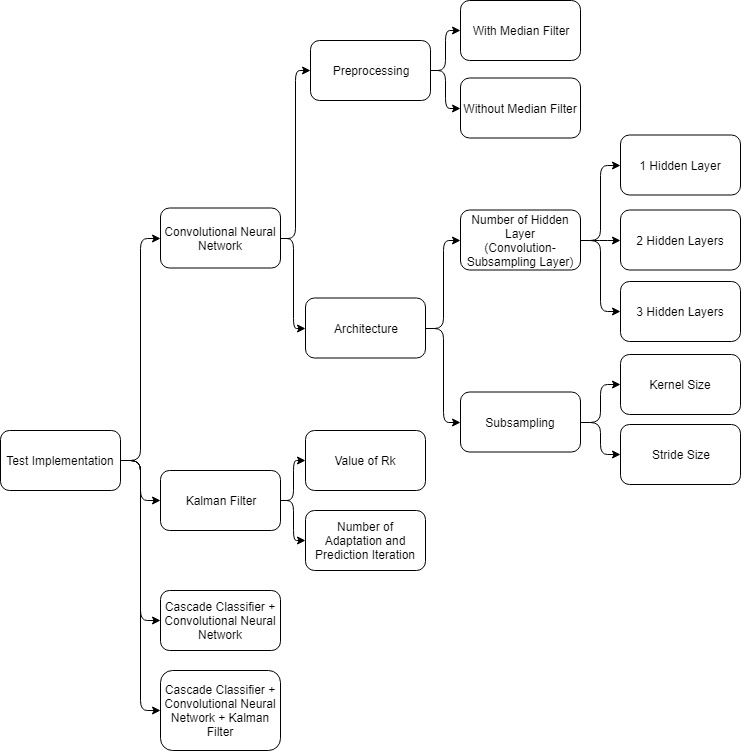
\includegraphics[width=13.5cm]{images/TestImplementation.jpg}}
%	\captionof{figure}{Diagram Pengujian Perangkat Lunak}
%	\label{fig:TestImplementation}
%\end{minipage}
%\end{adjustbox}
%
%\subsection{Tahap Pelatihan \textit{Convolutional Neural Network}}
%\noindent Pada tahap pelatihan \textit{Convolutional Neural Network} dilakukan pemilihan dan penggunaan citra sebagai data belajar. Berikut adalah algoritme untuk penentuan citra dari \textit{dataset}.
%\begin{spacing}{1}
%\noindent\rule{\textwidth}{1.5pt}
%\textbf{Algoritme Penentuan Citra dari \textit{Dataset}}
%\begin{enumerate}
%\item Muat berkas groundtruth.txt untuk \textit{dataset} yang berkaitan untuk mendapatkan seluruh posisi manusia  ($x_{1}$, $y_{1}$ dan $x_{2}$, $y_{2}$) dari setiap citra sebagai \textit{dataset} positif.
%\item Muat seluruh citra pada folder \textit{dataset} citra kedalaman dan dilakukan \textit{median filtering}.
%\item Potong dan lakukan penskalaan pada seluruh \textit{dataset} positif berdasarkan posisi manusia yang telah dimuat.
%\item Lakukan pengacakan posisi untuk \textit{dataset} negatif yang tidak berpotongan dengan posisi citra manusia dan dilanjutkan dengan pemotongan serta penskalaan agar ukuran seragam pada tahap \textit{Convolutional Neural Network}.
%\end{enumerate}
%\noindent\rule{\textwidth}{1pt}
%\end{spacing}
%\subsubsection{Normalisasi Nilai Citra}
%\noindent Normalisasi dilakukan untuk citra belajar agar memiliki rentang dari 0 hingga 1. Nilai citra awal memiliki rentang 0 hingga 255, sehingga untuk mendapatkan nilai pada rentang normalisasi dilakukan pembagian dengan nilai tertinggi yaitu 255. Proses normalisasi ini dilakukan agar pada saat tahap \textit{Convolutional Neural Network}, nilai citra sebagai masukan tidak terlalu tinggi pada saat dilakukannya \textit{backpropagation}. Digunakan rentang 0 hingga 1 karena menggunakan fungsi \textit{softmax} pada akhir lapisan \textit{Convolutional Neural Network}.\\
%
%\subsubsection{Nilai \textit{Kernel}}
%\noindent Untuk nilai inisialisasi \textit{kernel} pada \textit{Convolutional Neural Network}, digunakan nilai acak kecil dengan rentang -0.005 hingga 0.005. Nilai \textit{kernel} pada tahap inisialisasi bertujuan untuk membedakan fitur citra (\textit{menghilangkan sifat simetris pada jaringan}), sementara nilai \textit{kernel} kecil agar pada tahap pembelajaran dalam jaringan stabil atau tidak melompat jauh, dipengaruhi juga oleh nilai \textit{learning rate}. \textit{Kernel} tersebut berada pada lapisan \textit{Convolution} dan lapisan \textit{Fully Connected}. Jumlah \textit{kernel} pada setiap lapisan \textit{Convolution} hanya terdapat satu buah sementara lapisan \textit{Fully Connected} akan memiliki \textit{kernel} sebanyak jumlah kelas yaitu dua buah untuk kelas bukan manusia dan kelas manusia.\\
%
%\subsubsection{Nilai \textit{Learning Rate}}
%\noindent Salah satu \textit{hyperparameter} penting pada \textit{Convolutional Neural Network} adalah besar \textit{learning rate}. Nilai yang terlalu rendah menyebabkan lambatnya proses pembelajaran nilai \textit{kernel} untuk mencapai hasil optimal, yaitu akurasi tinggi dan nilai \textit{error} yang rendah. Sementara nilai yang terlalu tinggi akan membuat tidak stabil karena perubahan nilai \textit{kernel} yang tinggi. Nilai \textit{learning rate} yang optimal akan berbeda pada setiap kasus, namun umumnya digunakan nilai $10^{-3}$ dan semakin lama semakin kecil hingga $10^{-4}$. Pada penelitian ini akan diuji nilai $10^{-3}$ hingga $10^{-4}$. Selain itu, akan diberikan pula suatu konstanta yang akan membagi nilai \textit{learning rate} pada \textit{epoch} dengan kelipatan tertentu, sehingga semakin lama, nilai \textit{learning rate} semakin kecil dan akurasi akan semakin baik.\\
%
%\subsubsection{\textit{Stochastic Gradient Descent} (SGD)}
%\noindent \textit{Stochastic} atau \textit{on-line gradient descent} merupakan metode pembelajaran iteratif yang akan memperbarui nilai \textit{kernel} berdasarkan nilai turunan dari suatu data belajar pada penelitian ini adalah citra. Bila dibandingkan dengan \textit{batch gradient descent} (BGD), SGD akan lebih cepat dalam mendapatkan akurasi yang tinggi, hal ini disebabkan karena nilai SGD merupakan nilai yang \textit{noisy} hanya untuk sebuah data belajar, tidak seperti BGD yang mendapatkan nilai rata-rata pada seluruh data belajar dalam satu \textit{epoch}. Hal tersebut juga menyebabkan pembelajaran dengan SGD memiliki variansi tinggi dan memungkinkan untuk menemukan titik lokal minimum baru. Penelitian ini menggunakan metode pembelajaran menggunakan SGD karena lebih cepat dan lebih rendah dalam pemakaian memori daripada BGD, karena penelitian ini menggunakan jumlah citra yang banyak dan besar.\\
%
%\subsection{Metode Penyimpanan Model \textit{Convolutional Neural Network}}
%\noindent Penyimpanan model \textit{Convolutional Neural Network} pada penelitian ini digunakan kemampuan serialisasi objek dari Java, di mana objek direpresentasikan sebagai urutan \textit{byte} yang mencakup data objek beserta dengan informasi mengenai tipe data yang digunakan pada objek tersebut. Setelah dilakukan serialisasi objek dan disimpan sebagai berkas, berkas tersebut dapat dimuat kembali ke memori dengan melakukan deserialisasi objek. Untuk menyimpan objek yang telah diserialisasi digunakan kelas ObjectOutputStream, sementara untuk memuat dan melakukan deserialisasi digunakan kelas ObjectInputStream. Dengan kedua kelas tersebut, seluruh informasi pada objek dapat digunakan kembali dengan mudah.\\
%\noindent Untuk dapat menggunakan kemampuan serialisasi objek Java, seluruh kelas yang akan disimpan perlu mengimplementasikan \textit{interface} java.io.Serializable dan menentukan nilai dari variabel serialVersionUID secara manual. Nilai dari variabel tersebut akan menentukan pengaturan suatu objek pada saat diserialisasi atau dideserialisasi. Bila variabel tersebut tidak ditentukan secara eksplisit, Java dapat menginterpretasikan objek dengan nilai lain dan menyebabkan objek tidak dapat dimuat kembali.\\
%\noindent Model yang disimpan adalah objek dari kelas CNN.java yang telah dibuat. Karena nama ekstensi berkas dapat bervariasi, pada penelitian ini disimpan dengan ekstensi .cnn dan ketika dimuat kembali ke memori akan dimasukkan ke kelas CNN. Penyimpanan model akan dilakukan pada saat akurasi meningkat dan pada \textit{epoch} kelipatan tertentu agar dapat terlihat perubahan akurasi pada  \textit{epoch} tersebut. Kelipatan \textit{epoch} untuk menyimpan model ini sama dengan kelipatan \textit{epoch} untuk membagi nilai \textit{learning rate} pada penjelasan sebelumnya.\\
%
%\section{Pengujian \textit{Convolutional Neural Network} (CNN)}
%\noindent Arsitektur pengujian \textit{Convolutional Neural Network} menggunakan 2 pasang lapisan tersembunyi, yaitu \textit{convolution layer} di mana ukuran kernel adalah 5 $\times$ 5 dan \textit{stride} bernilai 1 berserta \textit{subsampling layer} dengan ukuran kernel 2 $\times$ 2 dan \textit{stride} sebesar 2. Lalu diakhiri dengan \textit{fully connected layer} yang \textit{kernel} memiliki ukuran. Pada setiap \textit{convolution layer} disertai dengan fungsi aktivasi dan hasil dari \textit{fully connected layer} akan dihitung menggunakan persamaan \textit{softmax} sehingga menghasilkan nilai antara 0 hingga 1 dan memiliki jumlah probabilitas total sebesar 1. \\
%\noindent Pengujian dilakukan dengan melakukan klasifikasi jenis citra berdasarkan posisi \textit{ground truth} yang diberikan dengan menentukan dan menguji jenis \textit{dataset}, besar \textit{epoch} maksimal, \textit{learning rate}, konstanta pembagi \textit{learning rate}, dan kelipatan \textit{epoch} untuk membagi \textit{learning rate} maupun untuk menyimpan model pelatihan. Hasil dari pengujian adalah akurasi yang dihasilkan pada \textit{epoch} tertentu.\\
%\noindent Secara garis besar pengujian akan dibagi dua yaitu pengujian pengaruh \textit{median filtering} dan pengujian arsitektur CNN. Setelah proses pelatihan dilakukan pengujian untuk melihat akurasi yang dihitung menggunakan persamaan \ref{eq:accuracy} dan waktu proses dalam satuan milidetik. Perhitungan waktu proses yang dilakukan hanya terhadap metode \textit{Convolutional Neural Network}, tanpa waktu untuk memuat \textit{dataset}, posisi, \textit{median filtering}, pemotongan, ataupun penskalaan citra.\\
%
%\subsection{Pengujian Pengaruh \textit{Median Filtering}}
%\noindent Berikut akan diuji dengan tahap \textit{preprocessing median filtering} 5 $\times$ 5 pada kedua jenis \textit{dataset} yang memiliki kondisi dan sudut pandang berbeda. Dilanjutkan dengan melakukan penskalaan citra agar memiliki ukuran seragam yaitu lebar 48 piksel dan tinggi 64 piksel. Dan akhirnya digunakan sebagai data belajar pada metode \textit{Convolutional Neural Network}. Hasil dari pembelajaran akan terdiri atas model dengan akurasi tertinggi dan model yang memiliki kelipatan \textit{epoch} 50. Ditentukan juga \textit{epoch} maksimal adalah 1.000. Seluruh model pembelajaran yang dihasilkan akan diuji sesuai dengan penjelasan dataset sebelumnya. Dengan catatan dataset negatif acak yang tidak berpotongan dengan citra manusia, memiliki ukuran asli (belum diubah skalanya) lebar 65 piksel, tinggi 80 piksel, dan \textit{stride} sebesar 15 piksel.\\
%
%\subsubsection{Pengujian terhadap \textit{Dataset Outdoor}}
%\noindent Pengujian berikut akan menggunakan nilai \textit{learning rate} awal sebesar 0,001, konstanta pembagi \textit{learning rate} 1,1287 dan 1,001 untuk setiap 50 \textit{epoch} dengan \textit{epoch} maksimal 1.000. Pada tabel \ref{tbl:TestOutdoor} terlihat hasil akurasi tertinggi dan akurasi rata-rata dengan masing-masing parameter. Nilai dengan akurasi tertinggi lebih banyak ditemukan bila menggunakan konstanta pembagi \textit{learning rate} 1,001 sementara nilai akurasi rata-rata lebih banyak bila menggunakan konstanta pembagi \textit{learning rate} 1,1287. Dan rata-rata waktu proses sebuah citra dari objek yang belum dikenali menggunakan CNN adalah 0.771 milidetik.
%\begin{table}[H]
%\centering
%\caption{Hasil Pengujian terhadap \textit{Dataset Outdoor}}
%\label{tbl:TestOutdoor}
%\begin{small}
%\begin{tabular}{|c|c|l|l|l|l|l|}
%\hline
%\multirow{2}{*}{\textbf{\begin{tabular}[c]{@{}c@{}}Initial\\ Learning Rate\end{tabular}}} & \multirow{2}{*}{\textbf{Divider}} & \multicolumn{1}{c|}{\multirow{2}{*}{\textbf{\begin{tabular}[c]{@{}c@{}}Outdoor/\\ folder\end{tabular}}}} & \multicolumn{2}{c|}{\textbf{Median Filter}}                               & \multicolumn{2}{c|}{\textbf{No Median Filter}}                            \\ \cline{4-7} 
%                                                                                       &                                   & \multicolumn{1}{c|}{}                                                                                              & \multicolumn{1}{c|}{\textbf{Average}} & \multicolumn{1}{c|}{\textbf{Max}} & \multicolumn{1}{c|}{\textbf{Average}} & \multicolumn{1}{c|}{\textbf{Max}} \\ \hline
%\multirow{6}{*}{0.001}                                                                 & \multirow{3}{*}{1.1287}           & Train 56                                                                                                           & 0.844681                              & 0.903904                          & 0.839609                              & 0.903904                          \\ \cline{3-7} 
%                                                                                       &                                   & Test 31                                                                                                            & \textbf{0.831169}                     & \textbf{0.880562}                 & \textbf{0.828094}                     & \textbf{0.87822}                  \\ \cline{3-7} 
%                                                                                       &                                   & Test 54                                                                                                            & \textbf{0.822849}                     & 0.865591                          & \textbf{0.818238}                     & 0.866935                          \\ \cline{2-7} 
%                                                                                       & \multirow{3}{*}{1.001}            & Train 56                                                                                                           & \textbf{0.859244}                     & \textbf{0.930931}                 & 0.849733                              & 0.921922                          \\ \cline{3-7} 
%                                                                                       &                                   & Test 31                                                                                                            & 0.825905                              & \textbf{0.880562}                 & 0.825332                              & \textbf{0.87822}                  \\ \cline{3-7} 
%                                                                                       &                                   & Test 54                                                                                                            & 0.815674                              & \textbf{0.870968}                 & 0.812254                              & \textbf{0.86828}                  \\ \hline
%\end{tabular}
%\end{small}
%\end{table}
%
%\noindent Perbandingan akurasi lebih rinci dari hasil pembelajaran dan pengujian menggunakan konstanta pembagi \textit{learning rate} 1,1287 dapat dilihat pada gambar \ref{fig:ComparisonTrain56_1.1287}, gambar \ref{fig:ComparisonTest31_1.1287}, dan gambar \ref{fig:ComparisonTest54_1.1287}. Terlihat pula untuk ketiga perbandingan tersebut tidak berbeda jauh.\\
%
%\begin{adjustbox}{width=1\textwidth}
%\noindent\begin{minipage}{\linewidth}
%	\framebox[\textwidth]{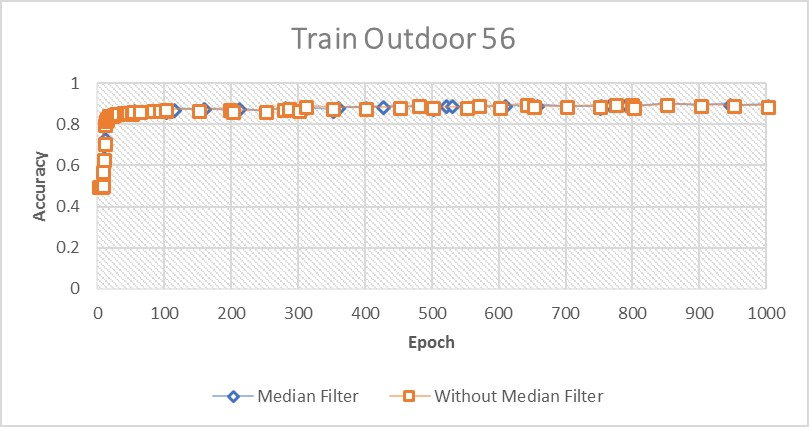
\includegraphics[width=10cm]{images/ComparisonTrain56_1,1287.jpg}}
%	\captionof{figure}{Perbandingan Akurasi dari Hasil Pembelajaran \textit{Dataset Outdoor} 56 dengan pembagi \textit{learning rate} 1,1287}
%	\label{fig:ComparisonTrain56_1.1287}
%\end{minipage}
%\end{adjustbox}
%
%\begin{adjustbox}{width=1\textwidth}
%\noindent\begin{minipage}{\linewidth}
%	\framebox[\textwidth]{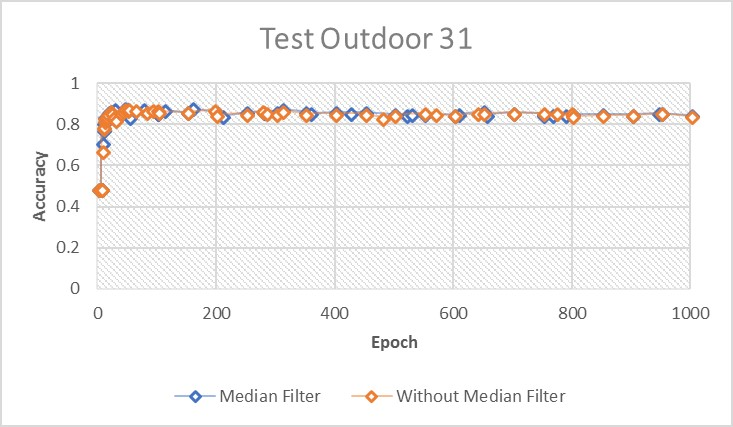
\includegraphics[width=10cm]{images/ComparisonTest31_1,1287.jpg}}
%	\captionof{figure}{Perbandingan Akurasi dari Hasil Pengujian \textit{Dataset Outdoor} 31 dengan pembagi \textit{learning rate} 1,1287}
%	\label{fig:ComparisonTest31_1.1287}
%\end{minipage}
%\end{adjustbox}
%
%\begin{adjustbox}{width=1\textwidth}
%\noindent\begin{minipage}{\linewidth}
%	\framebox[\textwidth]{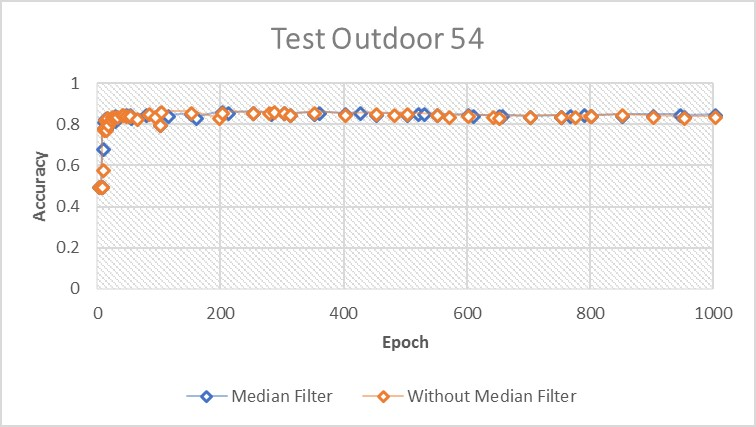
\includegraphics[width=10cm]{images/ComparisonTest54_1,1287.jpg}}
%	\captionof{figure}{Perbandingan Akurasi dari Hasil Pengujian \textit{Dataset Outdoor} 54 dengan pembagi \textit{learning rate} 1,1287}
%	\label{fig:ComparisonTest54_1.1287}
%\end{minipage}
%\end{adjustbox}
%
%\noindent Perbandingan akurasi lebih rinci dari hasil pembelajaran dan pengujian menggunakan konstanta pembagi \textit{learning rate} 1,001 dapat dilihat pada gambar \ref{fig:ComparisonTrain56_1.001}, gambar \ref{fig:ComparisonTest31_1.001}, dan gambar \ref{fig:ComparisonTest54_1.001}. Terlihat pula untuk ketiga perbandingan tersebut tidak berbeda jauh.\\
%
%\begin{adjustbox}{width=1\textwidth}
%\noindent\begin{minipage}{\linewidth}
%	\framebox[\textwidth]{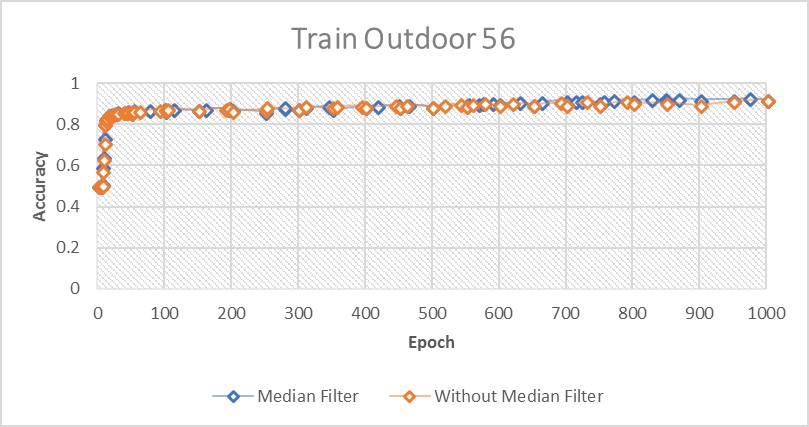
\includegraphics[width=10cm]{images/ComparisonTrain56_1,001.jpg}}
%	\captionof{figure}{Perbandingan Akurasi dari Hasil Pembelajaran \textit{Dataset Outdoor} 56 dengan pembagi \textit{learning rate} 1,001}
%	\label{fig:ComparisonTrain56_1.001}
%\end{minipage}
%\end{adjustbox}
%
%\begin{adjustbox}{width=1\textwidth}
%\noindent\begin{minipage}{\linewidth}
%	\framebox[\textwidth]{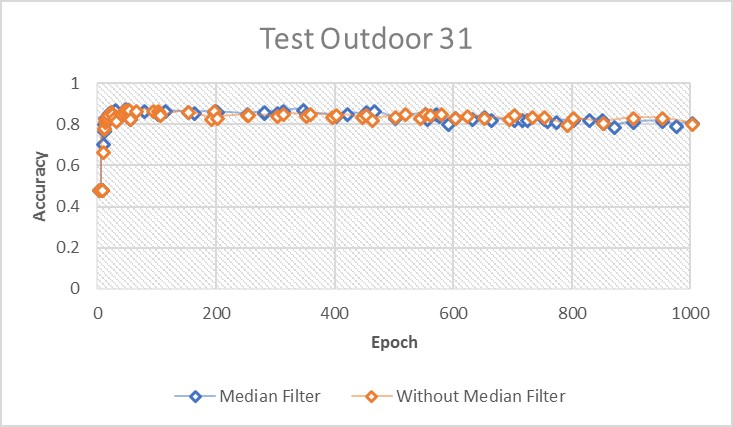
\includegraphics[width=10cm]{images/ComparisonTest31_1,001.jpg}}
%	\captionof{figure}{Perbandingan Akurasi dari Hasil Pengujian \textit{Dataset Outdoor} 31 dengan pembagi \textit{learning rate} 1,001}
%	\label{fig:ComparisonTest31_1.001}
%\end{minipage}
%\end{adjustbox}
%
%\begin{adjustbox}{width=1\textwidth}
%\noindent\begin{minipage}{\linewidth}
%	\framebox[\textwidth]{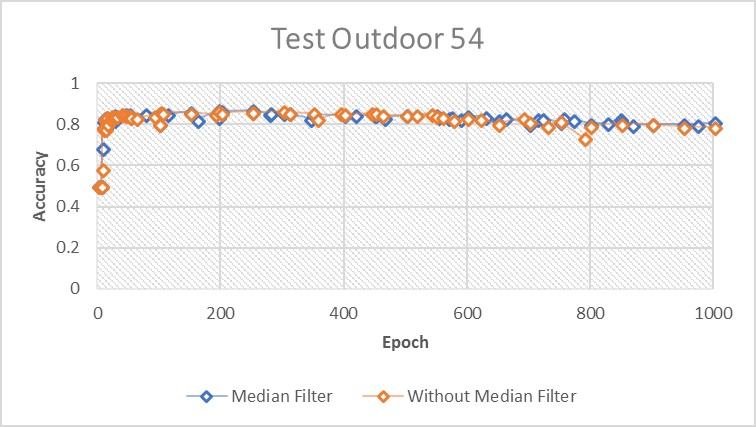
\includegraphics[width=10cm]{images/ComparisonTest54_1,001.jpg}}
%	\captionof{figure}{Perbandingan Akurasi dari Hasil Pengujian \textit{Dataset Outdoor} 54 dengan pembagi \textit{learning rate} 1,001}
%	\label{fig:ComparisonTest54_1.001}
%\end{minipage}
%\end{adjustbox}
%
%\noindent Berdasarkan pengujian dari kedua nilai konstanta pembagi \textit{learning rate} tersebut, terlihat bahwa dengan nilai 1,001 akan mendapatkan nilai akurasi tertinggi daripada nilai 1,1287 yang akan mengubah nilai \textit{learning rate} dalam rentang $10^{-3}$ hingga $10^{-4}$. Maka dalam pengujian selanjutnya akan digunakan nilai 1,001 sebagai konstanta pembagi \textit{learning rate}.
%
%\subsubsection{Pengujian terhadap \textit{Dataset Clothing Store}}
%\noindent Perbandingan nilai akurasi maksimal dan nilai rata-rata akurasi pada pengujian \textit{dataset clothing store} dapat dilihat pada tabel \ref{tbl:ComparisonCS}. Hasil perbandingan menunjukkan bahwa tanpa menggunakan \textit{median filter} menghasilkan akurasi yang jauh lebih baik daripada menggunakan \textit{median filter}. Nilai akurasi maksimum maupun nilai rata-rata akurasi pada pembelajaran dan kedua pengujian jauh lebih tinggi bila tidak menggunakan \textit{median filter}.
%\begin{table}[H]
%\centering
%\begin{small}
%\caption{Perbandingan hasil pengujian \textit{dataset clothing store} dengan pembagi \textit{learning rate} 1,001}
%\label{tbl:ComparisonCS}
%\begin{tabular}{|l|l|l|l|l|}
%\hline
%\multirow{2}{*}{Dataset Clothing Store/folder}                                         & \multicolumn{2}{c|}{\textbf{median filter}}                                      & \multicolumn{2}{c|}{\textbf{tanpa median filter}}                                \\ \cline{2-5} 
%                                        & \multicolumn{1}{c|}{\textbf{rata-rata}} & \multicolumn{1}{c|}{\textbf{maksimal}} & \multicolumn{1}{c|}{\textbf{rata-rata}} & \multicolumn{1}{c|}{\textbf{maksimal}} \\ \hline
%\multicolumn{1}{|l|}{Train CS} & 0.780535                                & 0.874936                               & \textbf{0.869531}                       & \textbf{0.895823}                      \\ \hline
%\multicolumn{1}{|l|}{Test CS}  & 0.685126                                & 0.807033                               & \textbf{0.777626}                       & \textbf{0.811321}                      \\ \hline
%\end{tabular}
%\end{small}
%\end{table}
%
%\noindent Perbandingan akurasi lebih rinci untuk hasil pembelajaran dan pengujian dapat dilihat pada gambar \ref{fig:ComparisonTrainCS} dan gambar \ref{fig:ComparisonTestCS}. Pada perbandingan ini terlihat bahwa dengan menggunakan \textit{median filtering}, pada \textit{epoch} awal akurasi naik namun turun hingga 70\% dan naik perlahan sementara tanpa menggunakan \textit{median filtering} tidak mengalami penurunan akurasi signifikan tersebut. Hal ini mungkin disebabkan oleh metode pembelajaran SGD yang kurang sesuai bila dilakukan \textit{median filtering}. Bila menggunakan \textit{median filtering}, \textit{Convolutional Neural Network} dengan SGD menemukan titik lokal minimum lain namun akurasinya berkisar pada 70\% saja.\\
%
%\begin{adjustbox}{width=1\textwidth}
%\noindent\begin{minipage}{\linewidth}
%	\framebox[\textwidth]{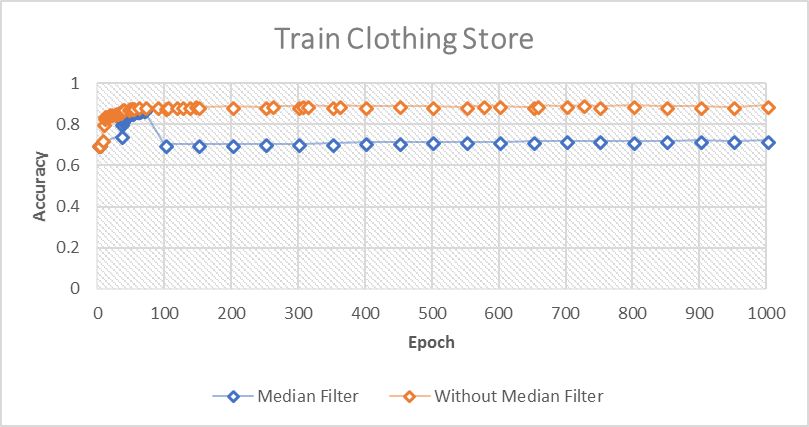
\includegraphics[width=10cm]{images/ComparisonTrainCS.jpg}}
%	\captionof{figure}{Perbandingan Akurasi dari Hasil Pembelajaran \textit{Dataset Clothing Store}}
%	\label{fig:ComparisonTrainCS}
%\end{minipage}
%\end{adjustbox}
%
%\begin{adjustbox}{width=1\textwidth}
%\noindent\begin{minipage}{\linewidth}
%	\framebox[\textwidth]{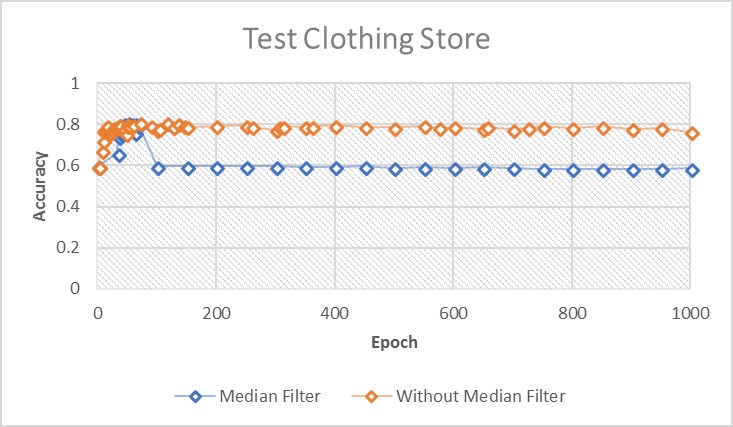
\includegraphics[width=10cm]{images/ComparisonTestCS.jpg}}
%	\captionof{figure}{Perbandingan Akurasi dari Hasil Pengujian \textit{Dataset Clothing Store}}
%	\label{fig:ComparisonTestCS}
%\end{minipage}
%\end{adjustbox}\\
%
%\subsection{Pengujian Arsitektur \textit{Convolutional Neural Network}}
%\noindent Pengujian berikut akan dilakukan perbandingan hasil bila dilakukan perubahan arsitektur yang digunakan pada metode CNN, yaitu berdasarkan jumlah lapisan tersembunyi dan \textit{hyperparameter} pada lapisan \textit{subsampling}.\\
%
%\subsubsection{Pengujian Jumlah Lapisan Tersembunyi}
%\noindent Pengujian dilakukan dengan menggunakan jumlah lapisan tersembunyi yang berbeda pada metode CNN. Hasil pengujian dengan maksimal \textit{epoch} 1.000 dapat dilihat pada tabel \ref{tbl:TestHiddenLayer}. Dapat disimpulkan bahwa menggunakan 1 lapisan tersembunyi untuk membedakan objek manusia pada citra kedalaman dapat dilakukan. Dan semakin banyak jumlah lapisan tersembunyi pada metode CNN, peningkatan akurasi akan naik lebih lambat, hal ini terlihat dari perbedaan nilai rata-rata akurasi karena terdapat lebih banyak nilai parameter atau bobot yang perlu dipelajari sehingga membutuhkan waktu dan \textit{epoch} yang juga lebih banyak.
%
%\begin{table}[H]
%\centering
%\caption{Hasil Pengujian Berdasarkan Jumlah Lapisan Tersembunyi}
%\label{tbl:TestHiddenLayer}
%\begin{small}
%\begin{tabular}{|l|l|l|l|}
%\hline
%\multicolumn{1}{|c|}{\textbf{Hidden Layer}} & \multicolumn{1}{c|}{\textbf{Outdoor/folder}} & \multicolumn{1}{c|}{\textbf{Average}} & \multicolumn{1}{c|}{\textbf{Max}} \\ \hline
%\multirow{3}{*}{1}                          & Train 56                                     & \textbf{0.941314}                     & \textbf{0.996997}                 \\ \cline{2-4} 
%                                            & Test 31                                      & \textbf{0.864413}                     & \textbf{0.903981}                 \\ \cline{2-4} 
%                                            & Test 54                                      & \textbf{0.8554}                       & 0.870968                          \\ \hline
%\multirow{3}{*}{2}                          & Train 56                                     & 0.859244                              & 0.930931                          \\ \cline{2-4} 
%                                            & Test 31                                      & 0.825905                              & 0.880562                          \\ \cline{2-4} 
%                                            & Test 54                                      & 0.815674                              & 0.870968                          \\ \hline
%\multirow{3}{*}{3}                          & Train 56                                     & 0.791383                              & 0.92993                           \\ \cline{2-4} 
%                                            & Test 31                                      & 0.758505                              & 0.873536                          \\ \cline{2-4} 
%                                            & Test 54                                      & 0.775396                              & \textbf{0.893817}                 \\ \hline
%\end{tabular}
%\end{small}
%\end{table}
%
%\subsubsection{Pengujian \textit{Hyperparameter} pada Lapisan \textit{Subsampling}}
%\noindent Berikut adalah pengujian dengan mengubah ukuran \textit{filter} dan \textit{stride} pada lapisan \textit{subsampling} yang juga memengaruhi dimensi metode \textit{Convolutional Neural Network}. Hasil dari pengujian tersebut dapat dilihat pada tabel \ref{tbl:TestPool}. Pengubahan arsitektur terlihat pada baris kedua, di mana S1 adalah lapisan \textit{subsampling} pertama, S2 adalah lapisan \textit{subsampling} kedua, F adalah ukuran \textit{filter}, dan S adalah ukuran \textit{stride}. Ditemukan hasil akurasi yang lebih tinggi untuk pengujian \textit{dataset outdoor} 31 pada arsitektur 1 dan pengujian \textit{dataset outdoor} 54 pada arsitektur 3.
%\begin{table}[H]
%\begin{small}
%\centering
%\caption{Hasil Akurasi Pengujian Arsitektur}
%\label{tbl:TestPool}
%\begin{tabular}{|l|l|l|l|l|l|l|l|l|}
%\hline
%\multicolumn{1}{|c|}{\multirow{3}{*}{\begin{tabular}[c]{@{}c@{}}Dataset\\ Outdoor\\/folder\end{tabular}}} & \multicolumn{2}{c|}{Arsitektur Awal}                                                                           & \multicolumn{2}{c|}{Arsitektur 1}                                                                    & \multicolumn{2}{c|}{Arsitektur 2}                                                                    & \multicolumn{2}{c|}{Arsitektur 3}                                                                    \\ \cline{2-9} 
%\multicolumn{1}{|c|}{}                                                                           & \multicolumn{2}{c|}{\begin{tabular}[c]{@{}c@{}}S1 (F = 2, S = 2),\\ S2 (F = 2, S = 2)\end{tabular}} & \multicolumn{2}{c|}{\begin{tabular}[c]{@{}c@{}}S1 (F = 4, S = 4),\\ S2 (F = 2, S = 2)\end{tabular}} & \multicolumn{2}{c|}{\begin{tabular}[c]{@{}c@{}}S1 (F = 4, S = 2),\\ S2 (F = 3, S = 2)\end{tabular}} & \multicolumn{2}{c|}{\begin{tabular}[c]{@{}c@{}}S1 (F = 6, S = 2),\\ S2 (F = 2, S = 2)\end{tabular}} \\ \cline{2-9} 
%\multicolumn{1}{|c|}{}                                                                           & \multicolumn{1}{c|}{\textbf{average}}              & \multicolumn{1}{c|}{\textbf{max}}              & \multicolumn{1}{c|}{\textbf{average}}              & \multicolumn{1}{c|}{\textbf{max}}              & \multicolumn{1}{c|}{\textbf{average}}              & \multicolumn{1}{c|}{\textbf{max}}              & \multicolumn{1}{c|}{\textbf{average}}              & \multicolumn{1}{c|}{\textbf{max}}              \\ \hline
%Train 56                                                                                         & \textbf{0.8593}                                  & \textbf{0.9309}                              & 0.7785                                        & 0.8829                                    & 0.7949                                         & 0.8879                                    & 0.8008                                        & 0.9009                                    \\ \hline
%Test 31                                                                                          & \textbf{0.8259}                                  & 0.8806                                       & 0.8002                                          & \textbf{0.8993}                             & 0.7782                                          & 0.8665                                      & 0.7295                                          & 0.808                                      \\ \hline
%Test 54                                                                                          & \textbf{0.8157}                                  & 0.871                                       & 0.7524                                          & 0.8522                                      & 0.7528                                          & 0.8616                                      & 0.7864                                          & \textbf{0.8817}                             \\ \hline
%\end{tabular}
%\end{small}
%\end{table}
%
%\section{Pengujian Kalman \textit{Filter}}
%\noindent Pengujian Kalman \textit{filter} dilakukan dengan cara membandingkan posisi \textit{ground truth dataset} terkait dengan hasil prediksi Kalman. \textit{Ground truth} tersebut telah diurutkan berdasarkan urutan manusia sehingga saat proses \textit{update} pada Kalman \textit{filter} data tidak tertukar. \textit{Dataset} pada pengujian ini menggunakan 15 citra dari \textit{dataset Outdoor 31} awal, karena pergerakan manusia pada citra tersebut berurutan (setelah diseleksi tidak ada yang citra yang dihapus). Akurasi pada pengujian ini dihitung menggunakan \textit{Jaccard Similarity} atau \textit{Intersection Over Union} (IoU) pada persamaan \ref{eq:JaccardSim} yaitu persentase perbandingan dari luas daerah yang berpotongan dengan gabungan luas dari kedua daerah.
%
%\noindent Pada gambar \ref{fig:UI} terlihat contoh tampilan hasil pada program yang berupa sekumpulan citra ditampilkan dalam waktu tertentu. Hasil dari pengujian Kalman \textit{filter} juga ditampilkan seperti pada contoh gambar \ref{fig:UI}.
%
%\begin{adjustbox}{width=1\textwidth}
%\noindent\begin{minipage}{\linewidth}
%	\framebox[\textwidth]{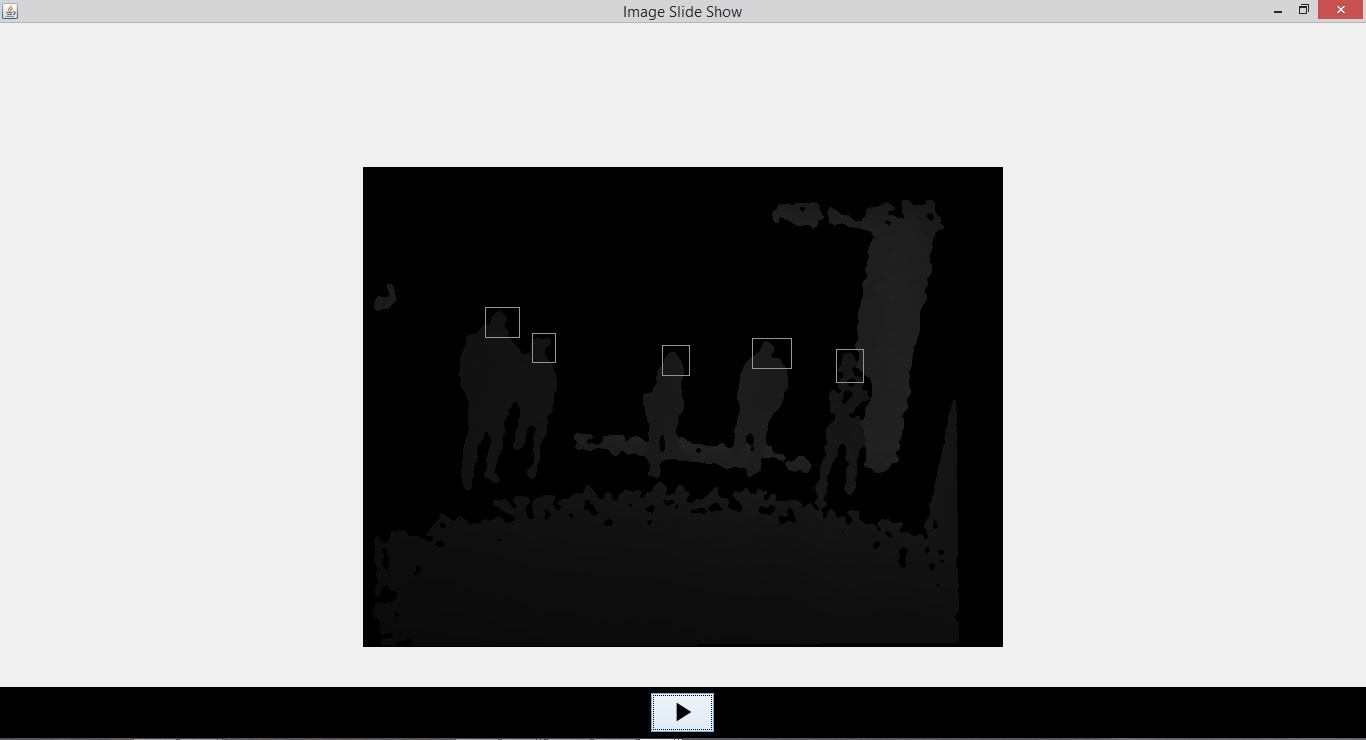
\includegraphics[width=13cm]{images/UI.JPG}}
%	\captionof{figure}{Contoh Tampilan Hasil Program}
%	\label{fig:UI}
%\end{minipage}
%\end{adjustbox}
%
%\subsection{Pengujian Kalman \textit{Filter} berdasarkan Nilai $r_{k}$}
%\noindent Pengujian berikut pada tabel \ref{TestKalmanRk} dilakukan untuk melihat pengaruh dari besar $r_{k}$ yang ditentukan terhadap akurasi. Dari hasil pengujian terlihat bahwa pada pergerakan manusia pada \textit{dataset} uji lebih baik menggunakan nilai $r_{k}$ yang bernilai kecil mendekati nilai 0, namun nilai $r_{k}$ yang lebih kecil dari 0,001 menghasilkan akurasi yang sama dengan nilai $r_{k}$ 0.001. Nilai $r_{k}$ yang kecil menghasilkan akurasi yang lebih tinggi, karena pergerakan setiap manusia pada dataset uji per citranya sedikit demi sedikit. Nilai $r_{k}$ menentukan secara tidak langsung menentukan seberapa jauh perbedaan dari kondisi sebelumnya dengan hasil prediksi pada waktu selanjutnya melalui nilai Kalman \textit{gain}.
%\begingroup
%\setlength{\LTleft}{-20cm plus -1fill}
%\setlength{\LTright}{\LTleft}
%\begin{small}
%\begin{longtable}{|l|l|}
%\caption{Pengujian Kalman \textit{filter} berdasarkan nilai $r_{k}$}
%\label{TestKalmanRk}\\
%\endfirsthead
%\multicolumn{2}{c}{\begin{tabular}[c]{@{}c@{}}\textbf{\tablename~\thetable} Pengujian Kalman \textit{filter}\\berdasarkan nilai $r_{k}$ (Lanjutan)\end{tabular}}\\
%\hline
%\multicolumn{1}{|c|}{\textbf{rk}} & \multicolumn{1}{c|}{\textbf{Accuracy}} \\ \hline
%\endhead
%\hline
%\multicolumn{1}{|c|}{\textbf{rk}} & \multicolumn{1}{c|}{\textbf{Accuracy}} \\ \hline
%0                                 & 0.108607172229742                      \\ \hline
%0.00001                           & 0.419061017161496                      \\ \hline
%0.0001                            & 0.419061017161496                      \\ \hline
%\textbf{0.001}                             & \textbf{0.419061017161496}                      \\ \hline
%0.002                             & 0.418925437955969                      \\ \hline
%0.004                             & 0.418475955655867                      \\ \hline
%0.006                             & 0.416588407850275                      \\ \hline
%0.008                             & 0.415225898891610                      \\ \hline
%0.01                              & 0.414088511175813                      \\ \hline
%0.02                              & 0.398183997549784                      \\ \hline
%0.03                              & 0.373033326741503                      \\ \hline
%0.04                              & 0.346114858983565                      \\ \hline
%0.05                              & 0.321034689670747                      \\ \hline
%0.06                              & 0.299162775024842                      \\ \hline
%\end{longtable}
%\end{small}
%\endgroup
%
%\subsection{Pengujian Kalman \textit{Filter} berdasarkan Jumlah Iterasi Adaptasi dan Prediksi}
%\noindent Pengujian Kalman berikut akan menguji akurasi dari jumlah iterasi untuk adaptasi dan jumlah iterasi untuk prediksi. Adaptasi dibutuhkan pada iterasi awal sebelum melakukan prediksi untuk mengumpulkan data dan mengurangi nilai kesalahan prediksi. Jumlah prediksi pun sebaiknya tidak terlalu banyak agar dapat menyesuaikan ulang berdasarkan posisi yang sesungguhnya.
%
%\noindent Gambar \ref{fig:GroundTruthKalman} adalah contoh tampilan dari hasil menggunakan posisi pada \textit{ground truth}. Posisi tersebut digunakan untuk iterasi adaptasi awal.
%
%\begin{adjustbox}{width=1\textwidth}
%\noindent\begin{minipage}{\linewidth}
%	\framebox[\textwidth]{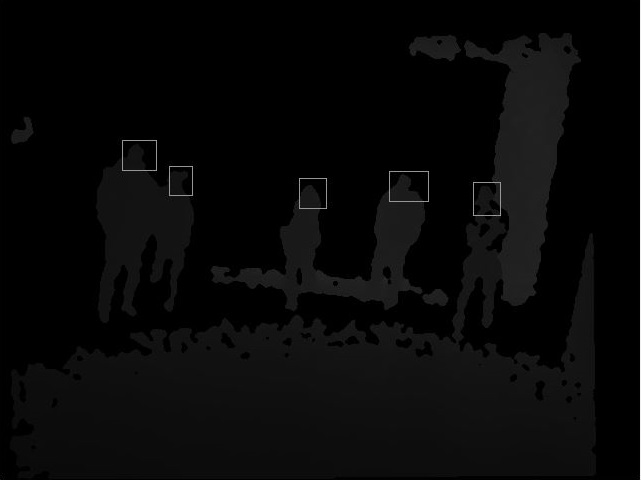
\includegraphics[width=10cm]{images/GroundTruthKalman.JPG}}
%	\captionof{figure}{Tampilan dari Menggunakan Posisi \textit{Ground Truth}}
%	\label{fig:GroundTruthKalman}
%\end{minipage}
%\end{adjustbox}
%
%\noindent Gambar \ref{fig:PredictionKalman} adalah contoh tampilan dari hasil prediksi Kalman \textit{filter}. Hasil posisi dari prediksi dilakukan setelah iterasi adaptasi. Untuk membedakan jenis proses, terlihat bahwa garis persegi panjang pada prediksi lebih tipis daripada pada saat adaptasi.
%
%\begin{adjustbox}{width=1\textwidth}
%\noindent\begin{minipage}{\linewidth}
%	\framebox[\textwidth]{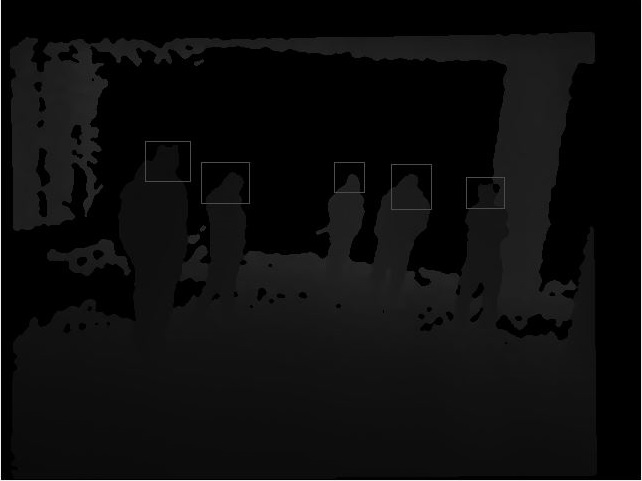
\includegraphics[width=10cm]{images/PredictionKalman.JPG}}
%	\captionof{figure}{Tampilan dari Hasil Prediksi Kalman \textit{filter}}
%	\label{fig:PredictionKalman}
%\end{minipage}
%\end{adjustbox}
%
%\noindent Tabel \ref{TestKalman} merupakan hasil pengujian, terlihat bahwa akurasi tertinggi 58,17\% dengan melakukan 3 iterasi adaptasi dan 2 iterasi prediksi.
%\begingroup
%\setlength{\LTleft}{-20cm plus -1fill}
%\setlength{\LTright}{\LTleft}
%\begin{small}
%\begin{longtable}{|l|l|l|l|}
%\caption{Pengujian Kalman \textit{filter}}
%\label{TestKalman}\\
%\endfirsthead
%\multicolumn{4}{c}{\textbf{\tablename~\thetable} Pengujian Kalman \textit{filter} (Lanjutan)} \\
%\hline
%\multicolumn{1}{|c|}{\textbf{Jumlah Manusia yang Diprediksi}} & \multicolumn{1}{c|}{\textbf{Adaptasi}} & \multicolumn{1}{c|}{\textbf{Prediksi}} & \multicolumn{1}{c|}{\textbf{Akurasi (IoU)}} \\ \hline
%\endhead
%\hline
%\multicolumn{1}{|c|}{\textbf{Jumlah Manusia yang Diprediksi}} & \multicolumn{1}{c|}{\textbf{Adaptasi}} & \multicolumn{1}{c|}{\textbf{Prediksi}} & \multicolumn{1}{c|}{\textbf{Akurasi (IoU)}} \\ \hline
%34                                            & 1                                         & 1                                      & 0.5280981346374015                          \\ \hline
%48                                            & 1                                         & 2                                      & 0.5407251792255828                          \\ \hline
%24                                            & 2                                         & 1                                      & 0.5508510824762379                          \\ \hline
%53                                            & 1                                         & 3                                      & 0.5114886186643478                          \\ \hline
%34                                            & 2                                         & 2                                      & 0.5446011086436996                          \\ \hline
%15                                            & 3                                         & 1                                      & 0.5710891939997309                          \\ \hline
%57                                            & 1                                         & 4                                      & 0.527003132775587                           \\ \hline
%42                                            & 2                                         & 3                                      & 0.567198009458369                           \\ \hline
%28                                            & \textbf{3}                                         & \textbf{2}                                      & \textbf{0.5817438475822965}                          \\ \hline
%14                                            & 4                                         & 1                                      & 0.57169235300142                            \\ \hline
%58                                            & 1                                         & 5                                      & 0.5370429178393978                          \\ \hline
%44                                            & 2                                         & 4                                      & 0.5546136307820144                          \\ \hline
%30                                            & 3                                         & 3                                      & 0.5156146672961023                          \\ \hline
%20                                            & 4                                         & 2                                      & 0.5200057238966823                          \\ \hline
%10                                            & 5                                         & 1                                      & 0.4849873175693231                          \\ \hline
%34                                            & 4                                         & 6                                      & 0.45175901936486573                         \\ \hline
%25                                            & 5                                         & 5                                      & 0.4254790605283677                          \\ \hline
%\end{longtable}
%\end{small}
%\endgroup
%
%\section{Pengujian \textit{Cascade Classifier} dengan \textit{Convolutional Neural Network}}
%\noindent Pengujian ini menggabungkan 2 metode yaitu \textit{Cascade Classifier} untuk lokalisasi mendapatkan kandidat posisi manusia dan \textit{Convolutional Neural Network} untuk klasifikasi kandidat citra yang didapatkan. Pengujian ini dihitung dengan \textit{confusion matrix} yaitu akurasi, \textit{precision}, dan \textit{recall}. Untuk citra yang memiliki nilai akurasi, \textit{precision}, atau \textit{recall} dibagi 0 akan dihapus dari perhitungan. Dalam pengujian ini digunakan \textit{threshold} probabilitas hasil \textit{Convolutional Neural Network} yang diterima adalah di atas 80\%.\\
%\noindent Pada gambar \ref{fig:CC} terlihat kandidat manusia yang telah dilokalisasi, ditandai dengan garis persegi panjang berwarna merah. Terdapat 5 kandidat posisi manusia yang memenuhi kriteria ukuran antara 40 $\times$ 40 hingga 90 $\times$ 90. Terdapat pula manusia yang tidak termasuk kandidat, disebabkan oleh citra belajar positif yang sedikit dan agak berbeda dengan citra pengujian. Sementara pada gambar \ref{fig:CCCNN} terlihat hasil klasifikasi manusia menggunakan \textit{Convolutional Neural Network} berdasarkan kandidat manusia yang diberikan. Dihasilkan 3 buah persegi panjang dengan warna hijau menandakan manusia dengan probabilitas di atas 80\%. \\
%\noindent Pengukuran waktu pengujian dilakukan pada 47 citra dalam \textit{dataset Outdoor} 31, dengan catatan waktu bila menggunakan \textit{median filter} adalah 21.558 milidetik atau 458,68 milidetik/citra, sementara tanpa menggunakan \textit{median filter} adalah 3.515 milidetik atau 74,79 milidetik/citra. Terlihat bahwa waktu proses tanpa menggunakan \textit{median filter} 6,13 kali lebih cepat daripada menggunakan \textit{median filter}. Perhitungan waktu tersebut dipengaruhi juga oleh jumlah kandidat yang dihasilkan oleh \textit{cascade classifier}.
%
%\begin{adjustbox}{width=1\textwidth}
%\noindent\begin{minipage}{\linewidth}
%	\framebox[\textwidth]{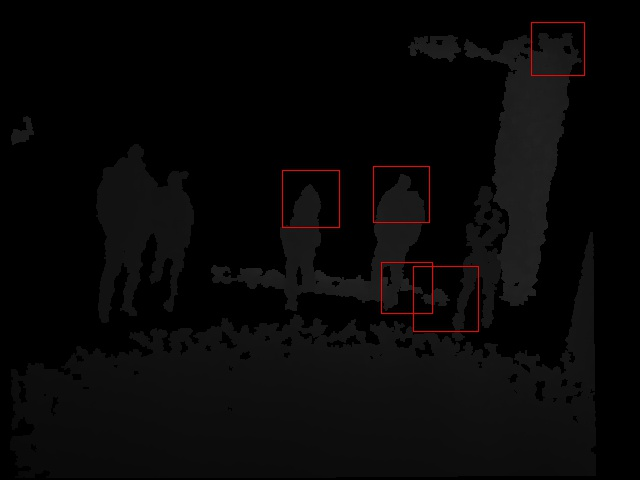
\includegraphics[width=10cm]{images/CC.JPG}}
%	\captionof{figure}{Contoh Lokalisasi \textit{Cascade Classifier}}
%	\label{fig:CC}
%\end{minipage}
%\end{adjustbox}
%
%\begin{adjustbox}{width=1\textwidth}
%\noindent\begin{minipage}{\linewidth}
%	\framebox[\textwidth]{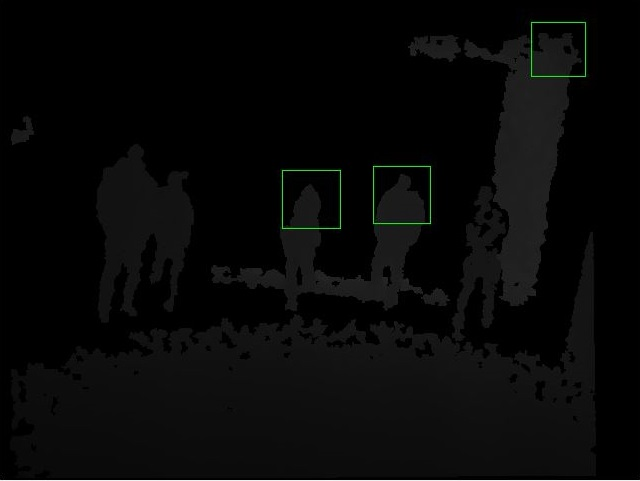
\includegraphics[width=10cm]{images/CCCNN.JPG}}
%	\captionof{figure}{Hasil Gabungan \textit{Cascade Classifier} dengan \textit{Convolutional Neural Network}}
%	\label{fig:CCCNN}
%\end{minipage}
%\end{adjustbox}
%
%\subsection{Pengujian terhadap \textit{Dataset Outdoor} 31}
%\noindent Tabel \ref{CCCNNTest31} merupakan hasil pengujian terhadap \textit{dataset Outdoor} 31. Pengujian ini menghasilkan rata-rata akurasi sebesar 79,97\%, rata-rata \textit{precision} sebesar 78,84\%, dan rata-rata \textit{recall} sebesar 94,93\%.
%\begingroup
%\setlength{\LTleft}{-20cm plus -1fill}
%\setlength{\LTright}{\LTleft}
%\begin{small}
%\begin{longtable}{|l|l|l|l|l|l|l|l|}
%\caption{Pengujian \textit{Cascade Classifier} dengan \textit{Convolutional Neural Network} pada \textit{Dataset Outdoor 31} \label{CCCNNTest31}}\\
%\hline
%\multicolumn{1}{|c|}{\textbf{Objek Terdeteksi}}                 & \textbf{TP} & \textbf{TN} & \textbf{FP} & \textbf{FN} & \textbf{Accuracy} & \textbf{Precision} & \textbf{Recall} \\ \hline
%\endfirsthead
%\multicolumn{8}{c}{\begin{tabular}[c]{@{}c@{}}\textbf{\tablename~\thetable} Pengujian \textit{Cascade Classifier} dengan \\\textit{Convolutional Neural Network} pada \textit{Dataset Outdoor 31} (Lanjutan)\end{tabular}}\\
%\hline
%\multicolumn{1}{|c|}{\textbf{Objek Terdeteksi}}                 & \textbf{TP} & \textbf{TN} & \textbf{FP} & \textbf{FN} & \textbf{Accuracy} & \textbf{Precision} & \textbf{Recall} \\ \hline
%\endhead
%5  & 2           & 2           & 1           & 0           & 0.8               & 0.666666667        & 1               \\ \hline
%4  & 3           & 0           & 1           & 0           & 0.75              & 0.75               & 1               \\ \hline
%3  & 2           & 0           & 0           & 1           & 0.666666667       & 1                  & 0.666666667     \\ \hline
%3  & 2           & 1           & 0           & 0           & 1                 & 1                  & 1               \\ \hline
%5  & 3           & 2           & 0           & 0           & 1                 & 1                  & 1               \\ \hline
%7  & 3           & 1           & 3           & 0           & 0.571428571       & 0.5                & 1               \\ \hline
%3  & 2           & 0           & 1           & 0           & 0.666666667       & 0.666666667        & 1               \\ \hline
%4  & 2           & 1           & 1           & 0           & 0.75              & 0.666666667        & 1               \\ \hline
%5  & 3           & 2           & 0           & 0           & 1                 & 1                  & 1               \\ \hline
%5  & 2           & 2           & 1           & 0           & 0.8               & 0.666666667        & 1               \\ \hline
%4  & 2           & 1           & 0           & 1           & 0.75              & 1                  & 0.666666667     \\ \hline
%6  & 4           & 2           & 0           & 0           & 1                 & 1                  & 1               \\ \hline
%4  & 2           & 1           & 1           & 0           & 0.75              & 0.666666667        & 1               \\ \hline
%4  & 2           & 1           & 1           & 0           & 0.75              & 0.666666667        & 1               \\ \hline
%5  & 2           & 1           & 2           & 0           & 0.6               & 0.5                & 1               \\ \hline
%3  & 2           & 1           & 0           & 0           & 1                 & 1                  & 1               \\ \hline
%3  & 2           & 1           & 0           & 0           & 1                 & 1                  & 1               \\ \hline
%3  & 2           & 0           & 1           & 0           & 0.666666667       & 0.666666667        & 1               \\ \hline
%3  & 2           & 1           & 0           & 0           & 1                 & 1                  & 1               \\ \hline
%5  & 3           & 0           & 2           & 0           & 0.6               & 0.6                & 1               \\ \hline
%5  & 1           & 1           & 2           & 1           & 0.4               & 0.333333333        & 0.5             \\ \hline
%1  & 1           & 0           & 0           & 0           & 1                 & 1                  & 1               \\ \hline
%2  & 1           & 0           & 1           & 0           & 0.5               & 0.5                & 1               \\ \hline
%2  & 1           & 0           & 1           & 0           & 0.5               & 0.5                & 1               \\ \hline
%2  & 2           & 0           & 0           & 0           & 1                 & 1                  & 1               \\ \hline
%1  & 1           & 0           & 0           & 0           & 1                 & 1                  & 1               \\ \hline
%5  & 3           & 1           & 1           & 0           & 0.8               & 0.75               & 1               \\ \hline
%5  & 3           & 1           & 1           & 0           & 0.8               & 0.75               & 1               \\ \hline
%5  & 3           & 1           & 1           & 0           & 0.8               & 0.75               & 1               \\ \hline
%4  & 3           & 1           & 0           & 0           & 1                 & 1                  & 1               \\ \hline
%4  & 2           & 1           & 1           & 0           & 0.75              & 0.666666667        & 1               \\ \hline
%2  & 2           & 0           & 0           & 0           & 1                 & 1                  & 1               \\ \hline
%4  & 2           & 1           & 1           & 0           & 0.75              & 0.666666667        & 1               \\ \hline
%3  & 1           & 1           & 0           & 1           & 0.666666667       & 1                  & 0.5             \\ \hline
%4  & 1           & 3           & 1           & 0           & 0.8               & 0.5                & 1               \\ \hline
%2  & 1           & 1           & 0           & 0           & 1                 & 1                  & 1               \\ \hline
%6  & 3           & 2           & 1           & 0           & 0.833333333       & 0.75               & 1               \\ \hline
%4  & 2           & 0           & 2           & 0           & 0.5               & 0.5                & 1               \\ \hline
%3  & 3           & 0           & 0           & 0           & 1                 & 1                  & 1               \\ \hline
%5  & 2           & 0           & 2           & 1           & 0.4               & 0.5                & 0.666666667     \\ \hline
%4  & 3           & 1           & 0           & 0           & 1                 & 1                  & 1               \\ \hline
%6  & 2           & 2           & 1           & 1           & 0.666666667       & 0.666666667        & 0.666666667     \\ \hline
%4  & 2           & 1           & 1           & 0           & 0.75              & 0.666666667        & 1               \\ \hline
%6  & 4           & 2           & 0           & 0           & 1                 & 1                  & 1               \\ \hline
%4  & 3           & 0           & 1           & 0           & 0.75              & 0.75               & 1               \\ \hline
%3  & 3           & 0           & 0           & 0           & 1                 & 1                  & 1               \\ \hline
%\multicolumn{5}{|c|}{\textbf{Average}}                                   & 0.799741201       & 0.788405797        & 0.949275362     \\ \hline
%\end{longtable}
%\end{small}
%\endgroup
%
%\subsection{Pengujian terhadap \textit{Dataset Outdoor} 54}
%\noindent Tabel \ref{CCCNNTest54} merupakan hasil pengujian terhadap \textit{dataset Outdoor} 54. Pengujian ini menghasilkan rata-rata akurasi sebesar 76,24\%, rata-rata \textit{precision} sebesar 76,88\%, dan rata-rata \textit{recall} sebesar 96,06\%.
%\begingroup
%\setlength{\LTleft}{-20cm plus -1fill}
%\setlength{\LTright}{\LTleft}
%\begin{small}
%\begin{longtable}{|l|l|l|l|l|l|l|l|}
%\caption{Pengujian \textit{Cascade Classifier} dengan \textit{Convolutional Neural Network} pada \textit{Dataset Outdoor 54}}
%\label{CCCNNTest54}\\
%\endfirsthead
%\multicolumn{8}{c}{\begin{tabular}[c]{@{}c@{}}\textbf{\tablename~\thetable} Pengujian \textit{Cascade Classifier} dengan \textit{Convolutional Neural Network} \\ pada \textit{Dataset Outdoor 54} (Lanjutan)\end{tabular}}\\
%\hline
%\multicolumn{1}{|c|}{\textbf{Objek Terdeteksi}}               & \multicolumn{1}{c|}{\textbf{TP}} & \multicolumn{1}{c|}{\textbf{TN}} & \multicolumn{1}{c|}{\textbf{FP}} & \multicolumn{1}{c|}{\textbf{FN}} & \multicolumn{1}{c|}{\textbf{Accuracy}} & \multicolumn{1}{c|}{\textbf{Precision}} & \multicolumn{1}{c|}{\textbf{Recall}} \\ \hline
%\endhead
%\hline
%\multicolumn{1}{|c|}{\textbf{Objek Terdeteksi}}               & \multicolumn{1}{c|}{\textbf{TP}} & \multicolumn{1}{c|}{\textbf{TN}} & \multicolumn{1}{c|}{\textbf{FP}} & \multicolumn{1}{c|}{\textbf{FN}} & \multicolumn{1}{c|}{\textbf{Accuracy}} & \multicolumn{1}{c|}{\textbf{Precision}} & \multicolumn{1}{c|}{\textbf{Recall}} \\ \hline
%4  & 2                                & 0                                & 2                                & 0                                & 0.5                                    & 0.5                                     & 1                                    \\ \hline
%2  & 2                                & 0                                & 0                                & 0                                & 1                                      & 1                                       & 1                                    \\ \hline
%1  & 1                                & 0                                & 0                                & 0                                & 1                                      & 1                                       & 1                                    \\ \hline
%2  & 2                                & 0                                & 0                                & 0                                & 1                                      & 1                                       & 1                                    \\ \hline
%3  & 2                                & 0                                & 1                                & 0                                & 0.666666667                            & 0.666666667                             & 1                                    \\ \hline
%3  & 2                                & 0                                & 1                                & 0                                & 0.666666667                            & 0.666666667                             & 1                                    \\ \hline
%2  & 2                                & 0                                & 0                                & 0                                & 1                                      & 1                                       & 1                                    \\ \hline
%4  & 2                                & 0                                & 2                                & 0                                & 0.5                                    & 0.5                                     & 1                                    \\ \hline
%5  & 1                                & 1                                & 2                                & 1                                & 0.4                                    & 0.333333333                             & 0.5                                  \\ \hline
%2  & 2                                & 0                                & 0                                & 0                                & 1                                      & 1                                       & 1                                    \\ \hline
%2  & 2                                & 0                                & 0                                & 0                                & 1                                      & 1                                       & 1                                    \\ \hline
%2  & 2                                & 0                                & 0                                & 0                                & 1                                      & 1                                       & 1                                    \\ \hline
%4  & 2                                & 1                                & 1                                & 0                                & 0.75                                   & 0.666666667                             & 1                                    \\ \hline
%1  & 1                                & 0                                & 0                                & 0                                & 1                                      & 1                                       & 1                                    \\ \hline
%1  & 1                                & 0                                & 0                                & 0                                & 1                                      & 1                                       & 1                                    \\ \hline
%3  & 1                                & 0                                & 1                                & 1                                & 0.333333333                            & 0.5                                     & 0.5                                  \\ \hline
%3  & 1                                & 1                                & 0                                & 1                                & 0.666666667                            & 1                                       & 0.5                                  \\ \hline
%1  & 1                                & 0                                & 0                                & 0                                & 1                                      & 1                                       & 1                                    \\ \hline
%1  & 1                                & 0                                & 0                                & 0                                & 1                                      & 1                                       & 1                                    \\ \hline
%3  & 2                                & 0                                & 1                                & 0                                & 0.666666667                            & 0.666666667                             & 1                                    \\ \hline
%3  & 2                                & 0                                & 1                                & 0                                & 0.666666667                            & 0.666666667                             & 1                                    \\ \hline
%3  & 2                                & 0                                & 1                                & 0                                & 0.666666667                            & 0.666666667                             & 1                                    \\ \hline
%3  & 2                                & 0                                & 1                                & 0                                & 0.666666667                            & 0.666666667                             & 1                                    \\ \hline
%5  & 2                                & 0                                & 3                                & 0                                & 0.4                                    & 0.4                                     & 1                                    \\ \hline
%2  & 1                                & 0                                & 1                                & 0                                & 0.5                                    & 0.5                                     & 1                                    \\ \hline
%3  & 1                                & 1                                & 1                                & 0                                & 0.666666667                            & 0.5                                     & 1                                    \\ \hline
%5  & 2                                & 1                                & 1                                & 1                                & 0.6                                    & 0.666666667                             & 0.666666667                          \\ \hline
%3  & 2                                & 0                                & 1                                & 0                                & 0.666666667                            & 0.666666667                             & 1                                    \\ \hline
%1  & 1                                & 0                                & 0                                & 0                                & 1                                      & 1                                       & 1                                    \\ \hline
%1  & 1                                & 0                                & 0                                & 0                                & 1                                      & 1                                       & 1                                    \\ \hline
%2  & 2                                & 0                                & 0                                & 0                                & 1                                      & 1                                       & 1                                    \\ \hline
%4  & 3                                & 1                                & 0                                & 0                                & 1                                      & 1                                       & 1                                    \\ \hline
%3  & 3                                & 0                                & 0                                & 0                                & 1                                      & 1                                       & 1                                    \\ \hline
%2  & 2                                & 0                                & 0                                & 0                                & 1                                      & 1                                       & 1                                    \\ \hline
%3  & 3                                & 0                                & 0                                & 0                                & 1                                      & 1                                       & 1                                    \\ \hline
%3  & 2                                & 0                                & 1                                & 0                                & 0.666666667                            & 0.666666667                             & 1                                    \\ \hline
%5  & 2                                & 0                                & 3                                & 0                                & 0.4                                    & 0.4                                     & 1                                    \\ \hline
%2  & 2                                & 0                                & 0                                & 0                                & 1                                      & 1                                       & 1                                    \\ \hline
%5  & 2                                & 0                                & 3                                & 0                                & 0.4                                    & 0.4                                     & 1                                    \\ \hline
%3  & 2                                & 0                                & 1                                & 0                                & 0.666666667                            & 0.666666667                             & 1                                    \\ \hline
%6  & 3                                & 1                                & 2                                & 0                                & 0.666666667                            & 0.6                                     & 1                                    \\ \hline
%4  & 2                                & 0                                & 1                                & 1                                & 0.5                                    & 0.666666667                             & 0.666666667                          \\ \hline
%3  & 3                                & 0                                & 0                                & 0                                & 1                                      & 1                                       & 1                                    \\ \hline
%4  & 4                                & 0                                & 0                                & 0                                & 1                                      & 1                                       & 1                                    \\ \hline
%4  & 3                                & 0                                & 1                                & 0                                & 0.75                                   & 0.75                                    & 1                                    \\ \hline
%3  & 2                                & 0                                & 1                                & 0                                & 0.666666667                            & 0.666666667                             & 1                                    \\ \hline
%4  & 2                                & 0                                & 2                                & 0                                & 0.5                                    & 0.5                                     & 1                                    \\ \hline
%3  & 1                                & 0                                & 2                                & 0                                & 0.333333333                            & 0.333333333                             & 1                                    \\ \hline
%3  & 2                                & 0                                & 1                                & 0                                & 0.666666667                            & 0.666666667                             & 1                                    \\ \hline
%1  & 1                                & 0                                & 0                                & 0                                & 1                                      & 1                                       & 1                                    \\ \hline
%2  & 2                                & 0                                & 0                                & 0                                & 1                                      & 1                                       & 1                                    \\ \hline
%3  & 2                                & 1                                & 0                                & 0                                & 1                                      & 1                                       & 1                                    \\ \hline
%5  & 2                                & 0                                & 3                                & 0                                & 0.4                                    & 0.4                                     & 1                                    \\ \hline
%3  & 1                                & 0                                & 2                                & 0                                & 0.333333333                            & 0.333333333                             & 1                                    \\ \hline
%1  & 1                                & 0                                & 0                                & 0                                & 1                                      & 1                                       & 1                                    \\ \hline
%\multicolumn{5}{|c|}{\textbf{Average}}         & 0.762424242                            & 0.768787879                             & 0.960606061                          \\ \hline
%\end{longtable}
%\end{small}
%\endgroup
%
%\section{Pengujian \textit{Cascade Classifier}, \textit{Convolutional Neural Network}, dengan Kalman \textit{Filter}}
%\noindent Pengujian ini menggabungkan keseluruhan metode yaitu \textit{Cascade Classifier}, \textit{Convolutional Neural Network}, dengan Kalman \textit{Filter}. Dalam pengujian ini digunakan \textit{threshold} probabilitas hasil \textit{Convolutional Neural Network} yang diterima adalah di atas 80\%. \textit{Dataset} yang digunakan adalah 15 citra dari \textit{dataset Outdoor 31} awal, karena pergerakan manusia pada citra tersebut berurutan (setelah diseleksi tidak ada yang citra yang dihapus). Waktu proses pengujian, menggunakan \textit{median filter} adalah 18.451 milidetik atau 392,57 milidetik/citra, sementara tanpa menggunakan \textit{median filter} adalah 2.049 milidetik atau 43,6 milidetik/citra. Terlihat bahwa tanpa menggunakan \textit{median filter} 9 kali lebih cepat daripada menggunakan \textit{median filter}.
%
%\noindent Pada gambar \ref{fig:CCCNNKalmanStart} terlihat proses iterasi adaptasi Kalman yang menggunakan data bukan dari \textit{ground truth}, melainkan posisi dari hasil \textit{Cascade Classifier} dan \textit{Convolutional Neural Network}.
%
%\begin{adjustbox}{width=1\textwidth}
%\noindent\begin{minipage}{\linewidth}
%	\framebox[\textwidth]{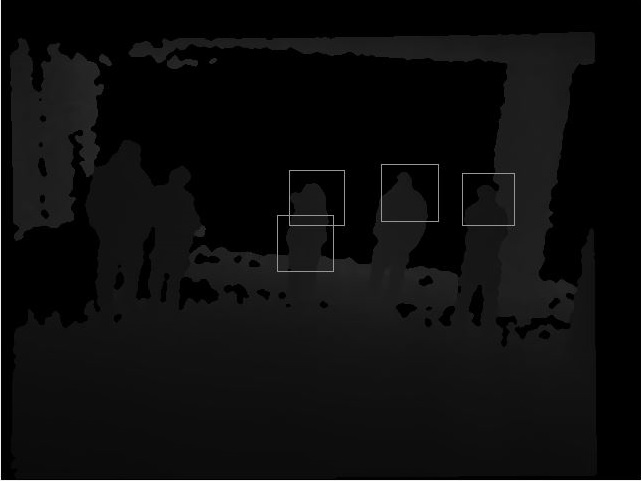
\includegraphics[width=10cm]{images/CCCNNKalmanStart.JPG}}
%	\captionof{figure}{Proses Adaptasi Kalman \textit{Filter} Menggunakan \textit{Cascade Classifier} dengan \textit{Convolutional Neural Network}}
%	\label{fig:CCCNNKalmanStart}
%\end{minipage}
%\end{adjustbox}
%
%\noindent Gambar \ref{fig:CCCNNKalman} merupakan hasil prediksi Kalman \textit{filter} setelah melakukan iterasi adaptasi. Hasil prediksi diberi garis persegi panjang yang lebih tipis daripada saat proses adaptasi.
%
%\begin{adjustbox}{width=1\textwidth}
%\noindent\begin{minipage}{\linewidth}
%	\framebox[\textwidth]{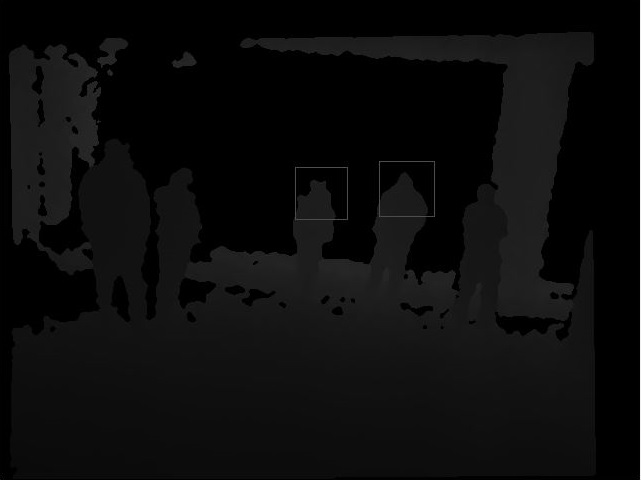
\includegraphics[width=10cm]{images/CCCNNKalman.JPG}}
%	\captionof{figure}{Hasil Prediksi Kalman \textit{Filter} Menggunakan \textit{Cascade Classifier} dengan \textit{Convolutional Neural Network}}
%	\label{fig:CCCNNKalman}
%\end{minipage}
%\end{adjustbox}
%
%\noindent Pada tabel \ref{CCCNNKalman} terlihat rata-rata akurasi sebesar 77,7\%, rata-rata \textit{precision} sebesar 79,44\%, dan rata-rata \textit{recall} sebesar 91,11\%. Sementara rata-rata waktu proses per citra adalah 5,388 milidetik.
%\begingroup
%\setlength{\LTleft}{-20cm plus -1fill}
%\setlength{\LTright}{\LTleft}
%\begin{small}
%\begin{longtable}{|l|l|l|l|l|l|l|l|}
%\caption{Pengujian \textit{Cascade Classifier}, \textit{Convolutional Neural Network}, dan Kalman \textit{filter}}
%\label{CCCNNKalman}\\
%\endfirsthead
%\multicolumn{8}{c}{\begin{tabular}[c]{@{}c@{}}\textbf{\tablename~\thetable} Pengujian \textit{Cascade Classifier} dengan \textit{Convolutional Neural Network} \\ , dan Kalman \textit{filter}\end{tabular}}\\
%\hline
%Jumlah Objek Terdeteksi                 & \multicolumn{1}{c|}{\textbf{TP}} & \multicolumn{1}{c|}{\textbf{TN}} & \multicolumn{1}{c|}{\textbf{FP}} & \multicolumn{1}{c|}{\textbf{FN}} & \multicolumn{1}{c|}{\textbf{Accuracy}} & \multicolumn{1}{c|}{\textbf{Precision}} & \multicolumn{1}{c|}{\textbf{Recall}} \\ \hline
%\endhead
%\hline
%\multicolumn{1}{|c|}{\textbf{Objek Terdeteksi}}                 & \multicolumn{1}{c|}{\textbf{TP}} & \multicolumn{1}{c|}{\textbf{TN}} & \multicolumn{1}{c|}{\textbf{FP}} & \multicolumn{1}{c|}{\textbf{FN}} & \multicolumn{1}{c|}{\textbf{Accuracy}} & \multicolumn{1}{c|}{\textbf{Precision}} & \multicolumn{1}{c|}{\textbf{Recall}} \\ \hline
%\multicolumn{1}{|l|}{ 5 } & 2           & 2           & 1           & 0           & 0.8               & 0.666667           & 1               \\ \hline
%\multicolumn{1}{|l|}{ 4 } & 3           & 0           & 1           & 0           & 0.75              & 0.75               & 1               \\ \hline
%\multicolumn{1}{|l|}{ 3 } & 2           & 0           & 0           & 1           & 0.666667          & 1                  & 0.666667        \\ \hline
%\multicolumn{1}{|l|}{ 3 } & 2           & 1           & 0           & 0           & 1                 & 1                  & 1               \\ \hline
%\multicolumn{1}{|l|}{ 5 } & 2           & 2           & 0           & 1           & 0.8               & 1                  & 0.666667        \\ \hline
%\multicolumn{1}{|l|}{ 7 } & 3           & 1           & 3           & 0           & 0.571429          & 0.5                & 1               \\ \hline
%\multicolumn{1}{|l|}{ 3 } & 2           & 0           & 1           & 0           & 0.666667          & 0.666667           & 1               \\ \hline
%\multicolumn{1}{|l|}{ 4 } & 2           & 1           & 1           & 0           & 0.75              & 0.666667           & 1               \\ \hline
%\multicolumn{1}{|l|}{ 5 } & 2           & 1           & 1           & 1           & 0.6               & 0.666667           & 0.666667        \\ \hline
%\multicolumn{1}{|l|}{ 5 } & 2           & 3           & 0           & 0           & 1                 & 1                  & 1               \\ \hline
%\multicolumn{1}{|l|}{ 4 } & 2           & 1           & 0           & 1           & 0.75              & 1                  & 0.666667        \\ \hline
%\multicolumn{1}{|l|}{ 6 } & 4           & 2           & 0           & 0           & 1                 & 1                  & 1               \\ \hline
%\multicolumn{1}{|l|}{ 4 } & 2           & 1           & 1           & 0           & 0.75              & 0.666667           & 1               \\ \hline
%\multicolumn{1}{|l|}{ 4 } & 2           & 1           & 1           & 0           & 0.75              & 0.666667           & 1               \\ \hline
%\multicolumn{1}{|l|}{ 5 } & 2           & 2           & 1           & 0           & 0.8               & 0.666667           & 1               \\ \hline
%\multicolumn{5}{|c|}{\textbf{Average}}                                                         & 0.776984          & 0.794444           & 0.911111        \\ \hline
%\end{longtable}
%\end{small}
%\endgroup
%
%\subsection{Perbandingan Hasil Pengujian}
%\noindent Berikut ini akan dibandingkan hasil pengujian bila hanya menggunakan metode \textit{Cascade Classifier} (CC) dan \textit{Convolutional Neural Network} (CNN) dan bila menambahkan Kalman \textit{filter} (KF) pada 15 citra awal \textit{dataset Outdoor} 31. Pada tabel \ref{tbl:HasilUjiPenggunaanKalman} terlihat bahwa tanpa Kalman \textit{filter} nilai akurasi dan nilai \textit{recall} lebih tinggi sementara nilai \textit{precision} lebih rendah daripada menggunakan Kalman \textit{filter}.
%\begin{table}[H]
%\centering
%\caption{Perbandingan Hasil Pengujian Penggunaan Kalman}
%\label{tbl:HasilUjiPenggunaanKalman}
%\begin{small}
%\begin{tabular}{l|l|l|l|}
%\cline{2-4}
%                                  & \multicolumn{3}{c|}{Average}                                                                 \\ \hline
%\multicolumn{1}{|c|}{Methods}     & \multicolumn{1}{c|}{Accuracy} & \multicolumn{1}{c|}{Precision} & \multicolumn{1}{c|}{Recall} \\ \hline
%\multicolumn{1}{|l|}{CC, CNN}     & \textbf{0.790317}             & 0.783333                       & \textbf{0.955556}           \\ \hline
%\multicolumn{1}{|l|}{CC, CNN, KF} & 0.776984                      & \textbf{0.794444}              & 0.911111                    \\ \hline
%\end{tabular}
%\end{small}
%\end{table}
%
%\noindent Selanjutnya, berdasarkan perbedaan dari waktu proses untuk melihat pengaruh dari penggunaan Kalman \textit{filter} terhadap waktu komputasi. Waktu pengujian pada seluruh citra dalam \textit{dataset outdoor} 31 yang telah dilakukan dengan satuan milidetik dapat dilihat pada tabel \ref{tbl:EfisiensiKomputasi}. Dengan menggunakan Kalman \textit{filter} waktu proses lebih cepat daripada tanpa Kalman \textit{filter}. Efisiensi komputasi dihitung dengan membandingkan selisih waktu dan waktu proses sebelum, yaitu tanpa mengunakan Kalman \textit{filter}. Efisiensi dari \textit{Kalman} pada pengujian menggunakan \textit{median filter} mempercepat komputasi 14,41\% sementara pada pengujian tanpa menggunakan \textit{median filter} mempercepat komputasi hingga 41,71\%.
%\begin{table}[H]
%\begin{small}
%\centering
%\caption{Perbandingan Waktu Pengujian dalam Milidetik}
%\label{tbl:EfisiensiKomputasi}
%\begin{tabular}{|l|l|l|l|l|}
%\hline
%\multicolumn{1}{|c|}{\multirow{2}{*}{Outdoor 31}} & \multicolumn{2}{c|}{median filtering}                           & \multicolumn{2}{c|}{tanpa median filter}                        \\ \cline{2-5} 
%\multicolumn{1}{|c|}{}                            & \multicolumn{1}{c|}{\begin{tabular}[c]{@{}c@{}}CC, CNN\\(ms)\end{tabular}} & \multicolumn{1}{c|}{\begin{tabular}[c]{@{}c@{}}CC, CNN, KF\\(ms)\end{tabular}} & \multicolumn{1}{c|}{\begin{tabular}[c]{@{}c@{}}CC, CNN\\(ms)\end{tabular}} & \multicolumn{1}{c|}{\begin{tabular}[c]{@{}c@{}}CC, CNN, KF\\(ms)\end{tabular}} \\ \hline
%Waktu proses 47 citra                             & 21558                                                                                                              & 18451                                                                                                                                & 3515                                                                                                               & 2049                                                                                                                                           \\ \hline
%Waktu per citra                                   & 458.6808511                                                                                                        & 392.5745                                                                                                                             & 74.78723404                                                                                                        & 43.59574                                                                                                                                       \\ \hline
%Efisiensi Komputasi                               &                                                                                                                    & 0.144123                                                                                                                             &                                                                                                                    & 0.41707                                                                                                                                        \\ \cline{1-1} \cline{3-3} \cline{5-5} 
%\end{tabular}
%\end{small}
%\end{table}

\newpage